\documentclass[a4paper,USenglish,cleveref,autoref,thm-restate,anonymous]{lipics-v2021}
%This is a template for producing LIPIcs articles. 
%See lipics-manual.pdf for further information.
%for A4 paper format use option "a4paper", for US-letter use option "letterpaper"
%for british hyphenation rules use option "UKenglish", for american hyphenation rules use option "USenglish"
%for section-numbered lemmas etc., use "numberwithinsect"
%for enabling cleveref support, use "cleveref"
%for enabling autoref support, use "autoref"
%for anonymousing the authors (e.g. for double-blind review), add "anonymous"
%for enabling thm-restate support, use "thm-restate"

%\graphicspath{{./graphics/}}%helpful if your graphic files are in another directory

\hideLIPIcs 

\ccsdesc{%
Theory of computation $\rightarrow$ 
Design and analysis of algorithms $\rightarrow$ 
Parameterized complexity and exact algorithms $\rightarrow$ 
Fixed parameter tractability}


% TODO 




\bibliographystyle{plainurl}
\newcommand{\citet}[1]{\cite{#1}}
\usepackage{graphicx}
\urlstyle{rm}
\def\UrlFont{\rm}
\usepackage{graphicx} 
\newif\iflong
\newif\ifshort

% comment the below line out for short version
\longtrue

\keywords{parameterized complexity, NLC-width, rank-width, decision trees, partially defined Boolean formulas}

\usepackage{tikz}
\usepackage{booktabs}
\usepackage[noend]{algpseudocode}
\usepackage{algorithm,algorithmicx}
\newcommand{\NULL}{\textnormal{\texttt{nil}}}
\newcommand{\TRUE}{\texttt{TRUE}}
\newcommand{\FALSE}{\texttt{FALSE}}

\algnewcommand\algorithmicinput{\textbf{Input:}}
\algnewcommand\INPUT{\item[\algorithmicinput]}

\algnewcommand\algorithmicoutput{\textbf{Output:}}
\algnewcommand\OUTPUT{\item[\algorithmicoutput]}

% decision trees and parameters
\newcommand{\DTL}{\probfont{DTS}}
\newcommand{\DTLh}{\probfont{DTD}}
\newcommand{\MSS}{\textup{MSS}}
\newcommand{\MNE}{\min_{\#}}
\newcommand{\GIL}{G^+_I}


\newcommand{\inst}{I}
\newcommand{\MIHS}{\probfont{MIHS}}

% \newcommand{\HD}{\delta}
% \newcommand{\MHD}{\delta_{\max}}
%\newcommand{\DMAX}{D_{\max}}

% \newcommand{\GD}{D}
% \newcommand{\IV}{I}

\usepackage{todonotes}
\presetkeys%
    {todonotes}%
    {inline,backgroundcolor=yellow}{}

%table stuff?
\usepackage{booktabs}
\usepackage{multirow}
%\usepackage{floatrow}

\usepackage{amsthm,amsmath,amssymb}
\usepackage{enumerate,verbatim}
\usepackage{xspace}

\usepackage{tikz,tikz-cd}
\usetikzlibrary{arrows,cd,positioning,shapes,patterns}


\usepackage[draft,author=]{fixme}
\fxsetup{theme=color}
%\newcommand{\todo}[1]{\fxerror{#1}}
\newcommand{\warn}[1]{\fxwarning{#1}}
\renewcommand{\note}[1]{\fxnote{#1}}
\newcommand{\nb}[1]{\todo{\scriptsize #1}}



\newcommand{\SB}{\{\,}
\newcommand{\SM}{\;{|}\;}
\newcommand{\SE}{\,\}}
\newcommand{\PP}{\mathcal{P}}
\newcommand{\QQ}{\mathcal{Q}}
\newcommand{\III}{\mathcal{I}}
\newcommand{\SSS}{\mathcal{S}}
\newcommand{\RRR}{\mathcal{R}}
\newcommand{\DDD}{\mathcal{D}}
\newcommand{\FFF}{\mathcal{F}}
\newcommand{\TTT}{\mathcal{T}}
\newcommand{\VVV}{\mathcal{V}}
\newcommand{\XXX}{\mathcal{X}}

\newcommand{\RR}{\mathcal{R}} 

\newcommand{\Z}{\mathbb{Z}}
\newcommand{\Nat}{\mathbb{N}}
\newcommand{\downcl}[2]{D_{#1}(#2)}
\newcommand{\pref}{P_{\leq^V}}
\newcommand{\suff}{S_{\leq^V}}

\newcommand{\bigoh}{\mathcal{O}}
\newcommand{\littleoh}{o}

 
 


\newcommand{\cc}[1]{{\mbox{\textnormal{\textsf{#1}}}}\xspace}  %% Complexity class
\newcommand{\cocc}[1]{{\mbox{\textrm{co}\textnormal{\textsf{#1}}}}\xspace}  %% Complexity class

\newcommand{\integers}{\mathbb{Z}}
\renewcommand{\P}{\cc{P}}
\newcommand{\NP}{\cc{NP}}
\newcommand{\coNP}{\cc{co-NP}}
\newcommand{\FPT}{\cc{FPT}}
\newcommand{\XP}{\cc{XP}}
\newcommand{\Weft}{{\cc{W}}}
\newcommand{\W}[1]{{\Weft}{{\textnormal[#1\textnormal]}}}
\newcommand{\paraNP}{\cc{paraNP}}
\newcommand{\paraNPs}{\cc{pNP}}


\newcommand{\fpt}{fixed-pa\-ra\-me\-ter trac\-ta\-ble\xspace}

\newcommand{\tuple}[1]{\langle{#1}\rangle}  % Tuple
\newcommand{\pn}[1]{\textsc{#1}}
\newcommand{\hy}{\hbox{-}\nobreak\hskip0pt}

%\newcommand{\citet}[1]{\citeauthor{#1}~\shortcite{#1}\xspace}
\newcommand{\nn}{\mathbb{N}}

\newcommand{\bigO}[1]{\ensuremath{{\mathcal O}(#1)}}
\newcommand{\bigOstar}[1]{\ensuremath{{\mathcal O}^*(#1)}}

\newcommand{\probfont}[1]{\textnormal{\textsc{#1}}}

%\newcommand{\stw}{dependency treewidth}



%\newcommand{\RAPROG}{\probfont{Proportionality Graph Allocation}}
\newcommand{\RAENVG}{\probfont{(Locally) Envy-Free Allocation}}
\newcommand{\RAENVGNL}{\probfont{Envy-Free Allocation}}
\newcommand{\RAENVGL}{\probfont{Locally Envy-Free Allocation}}

\newcommand{\EFA}{\textsc{EFA}}
\newcommand{\LEFA}{\textsc{LEFA}}

\newcommand{\FCGENVPROP}{envy-free}
\newcommand{\FCGENV}{locally envy-free}
\newcommand{\FCGPROP}{proportional}

\newcommand{\AT}{T_A}
\newcommand{\RT}{T_R}
\newcommand{\mundef}{\textup{undef}}
\newcommand{\BS}{\textup{BS}}

\newcommand{\RofRT}{R}
\newcommand{\RTBUN}{\textup{BUN}}
\newcommand{\RTVEC}{\vec{b}}
\newcommand{\RTVECSET}{\mathcal{B}}

\newcommand{\rall}{\alpha}
\newcommand{\itf}{\vec{u}}
\newcommand{\new}[1]{}
\newcommand{\valn}{\beta}
\newcommand{\VR}{\RRR}


\newcommand{\prop}[1]{#1}
\newcommand{\noprop}[1]{}
\newcommand{\bunmin}{\alpha_{\min}}
\newcommand{\bunmax}{\alpha_{\max}}
\newcommand{\propmax}{\beta}
\usepackage{boxedminipage}

\newcommand{\MCC}{\probfont{Multicolored Clique}}

\newcommand{\pbDef}[3]{%
\noindent
\begin{center}
\begin{boxedminipage}{0.98 \columnwidth}
#1\\[5pt]
\begin{tabular}{l p{0.70 \columnwidth}}
Input: & #2\\
Question: & #3
\end{tabular}
\end{boxedminipage}
\end{center}
}

\newcommand{\pbDefP}[4]{%
\noindent
\begin{center}
\begin{boxedminipage}{0.98 \columnwidth}
#1\\[5pt]
\begin{tabular}{l p{0.70 \columnwidth}}
Input: & #2\\
Parameter: & #3\\
Question: & #4
\end{tabular}
\end{boxedminipage}
\end{center}
}


\newcommand{\lc}{l}
\newcommand{\rc}{r}

\newcommand{\reaches}{r}


\newcommand{\CCC}{\mathcal{C}}

\newcommand{\ol}[1]{\overline{#1}}
\newcommand{\Card}[1]{|#1|}
\let\phi=\varphi
\let\epsilon=\varepsilon 
\def\hy{\hbox{-}\nobreak\hskip0pt} 
% Name for our encoding and for the whole approach
\newcommand{\enc}{DT\_pb}
\newcommand{\ench}{DT\_hyb}
\newcommand{\slv}{DT\_rec}
% Subsampling strategies
\newcommand{\stratrand}{RandSelect}
\newcommand{\stratlearn}{TreeSelect}
\newcommand{\stratleaf}{LeafSelect}
\newcommand{\stratinc}{MonotonicSelect}
% Feature reduction
\newcommand{\redcon}{\text{FR}}
\newcommand{\redgreedy}	{$\redcon_{\text{greedy}}$}
\newcommand{\redmaxsat}	{$\redcon_{\text{maxsat}}$}
\newcommand{\redrand}	{$\redcon_{\text{rand}}$}
\newcommand{\reddec}	{$\redcon_{\text{back}}$}

% reduction flags
\newcommand{\redinit}{RI}
\newcommand{\redinc}{RC}

\newcommand{\dif}{\text{\specialfont{diff}}}
\newcommand{\dom}{\text{\specialfont{dom}}}
\newcommand{\siz}{\text{\specialfont{size}}}
\newcommand{\solsize}{\text{\specialfont{sol}}}

\newcommand{\parameter}[1]{\text{\normalfont{\sffamily #1}}}
 

\newcommand{\var}{\text{\specialfont{feat}}}
\newcommand{\feat}{\text{\specialfont{feat}}}
\newcommand{\thres}{\lambda}

\newcommand{\leaf}{\text{\specialfont{leaf}}}



\newcommand{\specialfont}[1]{{\normalfont\slshape #1}}

\newcommand{\nlcw}{\text{\specialfont{nlcw}}}
\newcommand{\rtw}{\text{\specialfont{rtw}}}
\newcommand{\tw}{\text{\specialfont{tw}}}
\newcommand{\cw}{\text{\specialfont{cw}}}
\newcommand{\rw}{\text{\specialfont{rw}}}
\newcommand{\dep}{\text{\specialfont{dep}}}
\newcommand{\ghtw}{\text{\specialfont{ghtw}}}
\newcommand{\htw}{\text{\specialfont{htw}}}




\begin{document}
%\raggedright\pagestyle{empty}\nolinenumbers

\ifshort
\title{Fixed-Parameter Tractability of\\  Learning Small Decision Trees}
\fi
\iflong
\title{Fixed-Parameter Tractability of\\  Learning Small Decision Trees\\(full paper)}
\fi

\author{TODO}{~}{~}{}{}
\authorrunning{~}
\titlerunning{}
\maketitle


\begin{abstract}
We consider the NP-hard problem of finding a smallest decision tree which represents a given partially defined Boolean formula. We establish fixed-parameter tractability of the problem with respect to the NLC-width of the instance. We formulate a dynamic programming procedure which utilizes the NLC-decomposition of the instance. For this to work, we establish a succinct representation of partial solutions, so that the space and time requirements of each dynamic programming step remain bounded in terms of the NLC-width.
\end{abstract}
 
\newpage
\clearpage
\setcounter{page}{1}

\section{Introduction}
Decision trees have proved to be extremely useful tools for the describing, classifying, generalizing data~\cite{Larose05,Murthy98,Quinlan86}. In this paper, we consider decision trees for {\it classification instances (CIs)}, consisting of a finite set $E$ of {\it examples} (also called {\it feature vectors}) over a finite set $F$ of {\it features}. Each example $e\in E$ is a function $e:F\rightarrow \{0,1\}$ which determines whether the feature~$f$ is true or false for $e$.  Moreover, $E$ is given as a partition $E^+ \uplus E^-$ into positive and negative examples. For instance,  examples could represent medical patients and features diagnostic tests; a patient is positive or negative corresponding to whether they have been diagnosed with a certain disease or not. CIs are also called {\it partially} or {\it incompletely defined Boolean functions}, as we can consider the features as Boolean variables, and examples as  truth assignments that evaluate to 0 (for positive examples) or 1 (for negative examples). CIs have been studied as a key concept for the logical analysis of data and in switching theory \cite{BorosCHIKM11,Boros03,BorosGHIK95,BorosIbarakiMakino03,   CramaHammerIbaraki88,IbarakiCramaHammer11,Mccluskey65}.

Because of their simplicity, decision trees are particularly attractive for providing interpretable models of the underlying CI, an aspect whose importance has been strongly emphasized over the recent years~\cite{DarwicheHirth20,DoshivelezKim17,GoodmanFlaxman17,Lipton18,Monroe18}. In this context, one prefers {\it small trees}, as they are easier to interpret and require fewer tests to make a classification. Small trees are also preferred in view of the parsimony principle (Occam’s Razor) since small trees are expected to generalize better to new data~\cite{Bessiere09}. However, finding a small decision tree, as formulated in the following decision problem, is NP-complete~\cite{HyafilRivest76}. 

\begin{quote}
\probfont{Minimum Decision Tree Size (\DTL):} given a CI $E=E^+ \uplus E^-$ and an integer $s$, is there a decision tree with at most $s$ nodes for $E$?
\end{quote}

Given this complexity barrier, we propose a fixed-parameter algorithm for the problem, which exploits the input CI's hidden structure. The {\it incidence graph} of a CI is the bipartite graph $G_I(E)$ whose vertices are the examples on one side and the features on the other, where an example $e$ is adjacent with a feature $f$ if and only if $e(f)=1$. Figure~\ref{fig:example} shows a CI and a smallest decision tree for it, as well as the incidence graph.

\begin{figure}[b]
\small
\begin{minipage}{0.33\linewidth}
\centering
\begin{tabular}{@{}c@{~~}c@{~~}c@{~~}c@{~~}c@{}}
$E$  & $f_1$ & $f_2$ & $f_3$ & $f_4$ \\
\midrule
$e_1 \in E^-$ & 0 & 0 &1 & 0   \\
$e_2 \in E^-$ & 0 & 0 &1 & 1   \\
$e_3\in E^-$ & 0 & 1 &1 & 0 \\
$e_4\in E^-$ & 1 & 1 & 0 & 0   \\
$e_5\in E^+$ & 1 & 0 & 0 & 1  \\
$e_6\in E^+$ & 1 & 0 & 1 & 1  \\
\end{tabular}
\end{minipage}%
\begin{minipage}{0.33\linewidth}
\centering
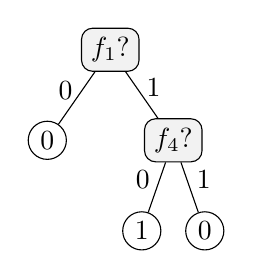
\begin{tikzpicture}[xscale=0.8,yscale=1.15]
\tikzstyle{test} = [draw, rectangle, rounded corners, fill=gray!10]
\tikzstyle{p} = [draw, circle, rounded corners, inner sep=2pt]
\tikzstyle{n} = [draw, circle, rounded corners, inner sep=2pt]
\draw  (0,0) node [test] (A) {$f_1$?}
(1,-1) node [test] (C) {$f_4$?}
(-1,-1) node [n] (B) {0}
(1.5,-2)  node [n] (E) {0}
(0.5,-2)  node [p] (D) {1};
\draw (A) -- (B) node [left,pos=0.35] {0};
\draw (A) -- (C) node [right,pos=0.35] {1};
\draw (C) -- (D) node [left,pos=0.35] {0};
\draw (C) -- (E) node [right,pos=0.35] {1};
\end{tikzpicture}
\end{minipage}%
\begin{minipage}{0.33\linewidth}
\centering
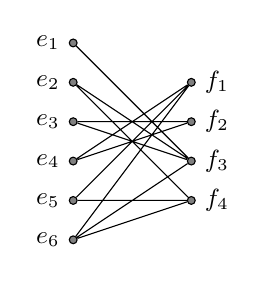
\begin{tikzpicture}[xscale=1.5,yscale=0.5]
\small
\tikzstyle{node} = [draw, circle, rounded corners, fill= gray, inner sep=1pt]
\draw
(0,0) node [node,label=left:$e_1$] (e1) {}
(0,-1) node [node,label=left:$e_2$] (e2) {}
(0,-2) node [node,label=left:$e_3$] (e3) {}
(0,-3) node [node,label=left:$e_4$] (e4) {}
(0,-4) node [node,label=left:$e_5$] (e5) {}
(0,-5) node [node,label=left:$e_6$] (e6) {}
(1,-1) node [node,label=right:$f_1$] (f1) {}
(1,-2) node [node,label=right:$f_2$] (f2) {}
(1,-3) node [node,label=right:$f_3$] (f3) {}
(1,-4) node [node,label=right:$f_4$] (f4) {}
(e1)--(f3) (e2)--(f3) (e2)--(f4) (e3)--(f2) (e3)--(f3) (e4)--(f1) (e4)--(f2) (e5)--(f1) (e5)--(f4) (e6)--(f1) (e6)--(f3) (e6)--(f4);
\end{tikzpicture}
\end{minipage}%
\caption{A CI $E=E^+\uplus E^-$ with six examples and four features (left), a decision tree with~5 nodes that classifies $E$ (middle), the incidence graph $G_I(E)$ (right).} \label{fig:example}
\end{figure}

Key to our algorithm are new notions for succinctly representing decision trees that correspond to subtrees of the incidence graph's tree decomposition.  Based on that, we can carry out a dynamic programming (DP) procedure along the tree decomposition.  

While the DP approach using treewidth is quite well understood and can often be quite easily designed for problems on graphs (or more generally problems whose solutions can be represented in terms of the graph for which the tree decomposition is given), the same DP approach can become rather involved if applied to problems whose solutions have
no or only minor resemblence to the graph for which one is given a tree decomposition. Probably the most prominent example for this is the celebrated result by Bodlaender~\cite{Bodlaender96}, where he uses a DP approach on an approximate tree decomposition to compute the exact treewidth of a graph; here, the solutions are tree decompositions, which are complex structures that cannot easily be represented in terms of the graph. Other prominent examples include a DP approach to compute the exact treedepth~\cite{DBLP:conf/icalp/ReidlRVS14} or clique-width~\cite{DBLP:journals/jgaa/EspelageGW03} using an optimal tree decomposition.  We face a similar problem, since solutions in our case are decision trees that do not bear any resemblence to the incidence graph for which we are given the tree decomposition. The main obstacle to overcome, therefore, is the design of the DP-records for our DP algorithm. That is, a record for a node $b$ in a tree decomposition for the incidence graph of $E$ needs to provide a compact representation of partial solutions, i.e. partial solutions in the sense that they represent the part of the solution for the whole instance $E$ that corresponds to the sub-instance induced by all features and examples contained in the bags in the subtree of the tree
decomposition rooted at the current node $b$. We overcome this obstacle in Section~\ref{sec:twfpt}, where we also provide intuitive descriptions and motivation for the definition of the records (Subsection~\ref{ssec:mainideas}).

\ifshort
{\it The full proof of statements marked with $(\star)$ can be found  in the full version of this paper.}
\fi

\section{Preliminaries}\label{chap:prelims}

\subsection{Parameterized Complexity}
We give some basic definitions of Parameterized Complexity and refer for a more in-depth treatment to other sources \cite{CyganFKLMPPS15,DowneyFellows13}. Parameterized complexity considers problems in a two-dimensional
setting, where a problem instance is a pair $(I,k)$, where $I$ is the main part and~$k$ is the parameter. A parameterized problem is {\it fixed-parameter tractable} if there exists a computable function $f$ such that instances $(I,k)$ can be solved in time $f(k) \|I\|^{O(1)}$.

\subsection{Graphs and NLC-width}

We will assume that the reader is familiar with basic graph theory (see, e.g. \cite{Diestel00,BangjensenGutin09}).  We
consider (vertex and edge labelled) undirected graphs. Let $G=(V,E)$
be an undirected graph. We write $V(G)=V$ and $E(G)=E$ for the sets of
vertices and edges of $G$, respectively. We denote an edge between $u
\in V$ and $v \in V$ as $\{u,v\}$. For a set $V' \subseteq V$ of
vertices we let $G[V']$ denote the graph induced by the vertices in
$V'$, i.e. $G[V']$ has vertex set $V'$ and edge set $E \cap \SB
\{u,v\} \SM u,v \in V' \SE$ and we let $G - V'$ denote the graph $G[V
\setminus V']$. For a set $E' \subseteq E$ of edges we let denote
$G-E'$ the graph with vertex set $V$ and edge set $E\setminus E'$.

\newcommand{\lab}{\lambda}

A \emph{$k$-graph} is a pair $(G,\lab)$, where
$G=(V,E)$ is an undirected graph and $\lab : V \rightarrow [k]$ is
a \emph{vertex label mapping} that labels every vertex $v \in V$ with
a label $\lab(v)$ from $[k]$. We call the $k$-graph consisting of exactly one vertex $v$ (say,
labeled by $i$) an \emph{initial $k$-graph} and denote it by $i(v)$.

Node label control-width (\emph{NLC-width}) is a graph parameter, defined as
follows~\cite{Wanke94}: Let $k \in \mathbb{N}$ be a positive
integer. An \emph{$k$-NLC-expression tree} of a graph $G=(V,E)$ is a subcubic tree
$B$, where every node $b$ of $B$ is associated with a $k$-graph (denoted by
$(G_b,\lab_b)$), such that:
\begin{enumerate}
\item Every leaf represents an initial $k$-graph $i(v)$ with $i \in
  [k]$ and $v \in V$.
\item Every non-leaf node $b$ with one child $c$ is a \emph{relabeling node}
  and is associated with a relabeling function $R_b:[k] \to
  [k]$. Moreover, $G_b$ is obtained from $G_c$ after relabelling all
  vertices of $G_c$ with label $i$ to label $R_b(i)$ for every $i \in [k]$.
\item Every non-leaf node $b$ with two children, i.e., a left child
  $l$ and a right child $r$, is a
  \emph{join node} and is associated with a \emph{join matrix}, i.e.,
  a binary $k\times k$ matrix
  $M_b$. Moreover, $(G_b,\lab_b)$ is obtained from the disjoint union of
  $(G_{l},\lab_l)$ and $(G_{r},\lab_r)$ after adding an edge from all vertices
  labeled $i$ in $G_{l}$ to all vertices labeled $j$ in $G_{r}$ whenever $M_b[i,j]=1$.
\item $G$ is equal to the $G_r$ for the root node $r$ of $B$.
\end{enumerate}

The NLC-width of a graph~$G$, denoted by~$\nlcw(G)$, is the
minimum~$k$ for which~$G$ has a $k$-NLC-expression tree.
A $k$-NLC-expression tree is {\it nice} if every relabelling node has
a relabelling function $R:[k] \to [k]$ such that for some $i,j \in
[k]$, $R(i)=j$ and $R(\ell)=\ell$ for all $\ell \in [k] \setminus
\{i\}$. Clearly, given a $k$-NLC-expression tree, a nice
$k$-NLC-expression tree can be found in polynomial time; simply replace
every relabelling node (that relabels more than one label at a time)
by a sequence of relabelling nodes.

Let~$b$ be a node in a $k$-NLC-expression tree of a graph~$G$.
We denote by $V_b$ the set of vertices of $G_b$.
%KD: Possibly wnat to prove this/provide a reference.
By the definition of a $k$-NLC-expression tree, if $u,v \in V_b$ have
the same label in $(G_b,\lab_b)$ and $w \in V(G) \setminus V_b$, then~$u$ is adjacent to~$w$ in $G$ if and only if~$v$ is.

%KD: TODO: Compare to clique-width/rank-width.
Computing the NLC-width of a graph is NP-hard~\cite{GW05}.
However, it is sufficient to use the algorithm of Seymour and Oum~\cite{OS06}, which returns a $c$-expression for some $c\leq 2^{3\cw(G)+2}-1$ in $O(n^9\log n)$ time, or the later improvements of Oum~\cite{Oum08} and Hlin\v{e}n\'y and Oum~\cite{HO08} that provide cubic-time algorithms which yield a $c$-expression for some $c\leq 8^{\cw(G)}-1$ and $c\leq 2^{\cw(G)+1}-1$, respectively.

\subsection{Classification Problems} 
An {\it example} $e$ is a function $e:\feat(e) \rightarrow \{0,1\}$ defined on a finite set $\feat(e)$ of {\it features}. For a set $E$ of examples, we put $\feat(E)=\bigcup_{e\in E} \feat(e)$. We say that two examples $e_1,e_2$ {\it agree} on a feature $f$ if $f \in \feat(e_1)$, $f\in \feat(e_2)$ and $e_1(f)=e_2(f)$. If $f \in \feat(e_1)$, $f \in \feat(e_2)$ but $e_1(f)\neq e_2(f)$, we say that the examples {\it disagree on $f$}.

A {\it classification instance (CI)} (also called a {\it partially defined Boolean function}\ \cite{IbarakiCramaHammer11})
$E=E^+ \uplus E^-$ is the disjoint union of two sets of examples, where for all $e_1,e_2\in E$ we have $\feat(e_1)=\feat(e_2)$. The examples in $E^+$ are said to be {\it positive}; the examples in $E^-$ are said to be {\it negative}.  A set $X$ of examples is {\it uniform} if $X\subseteq E^+$ or $X \subseteq E^-$; otherwise $X$ is {\it non-uniform}.
 
Given a CI $E$, a subset $F\subseteq \feat(E)$ is a {\it support set} of $E$ if any two examples $e_1\in E^+$ and $e_2\in E^-$ disagree in at least one feature of $F$.  Finding a smallest support set, denoted by $\MSS(E)$, for a classification instance $E$ is an NP-hard task~\cite[Theorem 12.2]{IbarakiCramaHammer11}.
 
We define the {\it incidence graph} of $E$, denoted by $G_I(E)$, as the bipartite graph with partition $(E, \feat(E))$ having an edge between an example $e \in E$ and a feature $f\in \feat(e)$ if $f(e)=1$.

\subsection{Decision Trees}
A {\it decision tree} (DT) (or {\it classification tree}) is a rooted tree $T$ with vertex set $V(T)$ and arc set $A(T)$, where each non-leaf node (called a {\it test}) $v\in V(T)$ is labelled with a feature $\feat(v)$, each non-leaf node $v$ has exactly two out-going arcs, a {\it left arc} and a {\it right arc}, and each leaf is either a {\it positive} or a {\it negative} leaf. We write $\feat(T)=\SB v\in V(T) \SM \feat(v) \SE$.

Consider a CI $E$ and a decision tree $T$ with $\feat(T)\subseteq \feat(E)$. For each node $v$ of $T$ we define $E_T(v)$ as the set of all examples $e\in E$ such that for each left (right, respectively) arc $(u,v)$ on the unique path from the root of $T$ to~$v$ we have $e(\feat(v))=0$ ($e(\feat(v))=1$, respectively).  $T$ {\it correctly classifies} an example $e\in E$ if $e$ is a positive (negative) example and $e\in E_T(v)$ for a positive (negative) leaf. We say that $T$
{\it classifies} $E$ (or simply that $T$ is a DT for $E$) if $T$ correctly classifies every example $e \in E$. See Figure~\ref{fig:example} for an illustration of a CI, its incidence graph, and a DT that classifies $E$.

The size of $T$ is its number of nodes, i.e. $|V(T)|$. We consider the following problem.

\pbDef{\probfont{Minimum Decision Tree Size} (\DTL)}{A classification instance $E$ and an integer $s$.}{Is there a decision tree of size at most $s$ for $E$?}

We now give some simple auxiliary lemmas that are required by our algorithm.

\begin{lemma}\label{lem:enum-dt-fund}
Let $A$ be a set of features of size $a$. Then the number of DTs of size at most $s$ that use only features in $A$ is at most $a^{2s+1}$ and those can be enumerated in $\bigoh(a^{2s+1})$ time.
\end{lemma}

\begin{proof}
We start by counting the number of trees $T$ with $n$ nodes that can potentially underlie a DT with $n$ nodes. Note that there is one-to-one correspondence between trees $T$ that underlie a DT with $n$ nodes and unlabelled rooted ordered binary trees with $n$ nodes (where ordered refers to an ordering of the at most $2$ child nodes). Since it is known that the number of unlabelled rooted ordered binary trees with $n$ nodes is equal to the $n$-th Catalan number $C_n$ and that those trees can be enumerated in $\bigoh(C_n)$ time~\cite{stanley2015catalan}, we already obtain that we can enumerate all of the at most $C_n$ possible trees $T$ underlying a DT of size $n$ in $\bigoh(C_n)$ time. Therefore, there are at most $sC_{s}$ possible trees of size at most $s$ that can underlie a DT with at most $s$ nodes and those can be enumerated in $\bigoh(sC_{s})$ time. It now remains to bound the number of possible feature assignments $\feat(f)$ for these trees as well as the number of possibilities for the leave nodes that can be either labelled positive or negative. Since we can assume that $a\geq 2$, we obtain that the number of possible feature assignments (and labellings of leaf-nodes) of a tree $T$ with $n$ nodes is at most $a^n$. Taking everything together, we obtain that there are at most $sC_sa^s \leq s4^sa^s \leq a^{2s+1}$ many DTs of size at most $s$ using only features in $A$ and those can be enumerated in $\bigoh(a^{2s+1})$ time. 
\end{proof}

\begin{lemma}\label{lem:enum-dt}
Let $A$ be a set of features of size $a$. There are at most $a^{2^{a+1}+3}$ inclusion-wise minimal DTs using only features in $A$ and these can be enumerated in $\bigoh(a^{2^{a+1}+3})$ time.
\end{lemma}

\begin{proof}
Note that an inclusion-wise minimal DT $T$ that uses only features in $A$ has at most $2^a+1$ nodes; this is because every feature appears at most once on every path $T$. Therefore, we obtain from Lemma~\ref{lem:enum-dt-fund} that the number of choices for $T$ is at most $a^{2(2^a+1)+1}=a^{2^{a+1}+3}$.
\end{proof}

\newcommand{\NO}{\textbf{NO}}
\newcommand{\TsmDT}{(2^{|E|})^{4|E|-1}}

\begin{lemma}\label{lem:comsmallDT}
Let $E$ be a CI. Then one can decide whether $E$ has a DT and if so output a DT of minimum size for $E$ in time $\bigoh(\TsmDT)$.
\end{lemma}

\begin{proof}
Note first that $|\feat(E)|\leq 2^{|E|}$ since we can assume that $E$ does not contain two equivalent features. Moreover, $E$ has a DT if and only if $\feat(E)$ is a support set, which can be checked in time $\bigoh(|E|^2|\feat(E)|)$ by checking, for every pair of positive and negative examples in $E$, whether there is a feature that distinguishes them. If this is not the case, we output \NO{}, so assume that $E$ has a DT. Note that any inclusion-wise minimal DT for $E$ has at most $|E|$ leaves and therefore size at most $2|E|-1$. We can therefore employ Lemma~\ref{lem:enum-dt-fund} to enumerate all inclusion-wise minimal potential DTs for $E$ in time $\bigoh((2^{|E|})^{2(2|E|-1)+1}) \in \bigoh(\TsmDT)$. For every such tree we then check whether it is indeed a DT for $E$ and return a DT for $E$ of minimum size found during this process.
\end{proof}

\newcommand{\exam}{\text{\specialfont{exam}}}

\section{An FPT-Algorithm for NLC-width}\label{sec:twfpt}

\newcommand{\afs}{\textup{TF}}
\newcommand{\afsF}{\textup{TF}_F}
\newcommand{\afsP}{\textup{TF}_P}
\newcommand{\addF}{\oplus}

In this section, we present our main result, i.e. we will show that \DTL{} is fixed-parameter tractable parameterized by 
NLC-width.

\begin{theorem}\label{the:trac-nlcw-b-td}
  Let $E$ be a CI, let $B$ be an NLC-decomposition of width $\omega$ for
  $G_I(E)$, and let $s$ be an integer. Then, deciding whether $E$ has a
  DT of size at most $s$ is fixed-parameter tractable parameterized by
  $\omega$.
\end{theorem}

\note{todo: Due to proposition ...}

\begin{corollary}\label{cor:trac-tw-b}
  \DTL{} is fixed-parameter tractable parameterized by NLC-width.
\end{corollary}

In principle, we will use a dynamic programming algorithm along the
NLC-decomposition $(B,\chi)$ of $G_I(E)$ that computes a set of records
for every node $b$ of $B$ in a bottom-up manner. Each record will
represent an equivalence class of solutions (DTs) for the whole
instance restricted to the examples and features contained in the
current subtree rooted in $b$, i.e. the examples and features
contained in $\chi(b)$. Before we continue with the formal notions
and definitions required to define the records, we want to illustrate
the main ideas and motivations. In what follows let $B$ be an
NLC-decomposition of $G_I(E)$ of width $k$. For $b
\in V(B)$, we write $\feat(b)$ and $\exam(b)$ for the sets
$\chi(b)\cap\feat(E)$ and $\chi(b)\cap E$, respectively. 


\subsection{Description of the Main Ideas Behind the
  Algorithm} \label{ssec:mainideas}
\note{todo: adjust to NLC-width}

Consider a node $b$ of $B$. To simplify the presentation, we will sometime refer to the features and examples in $\chi(B_b)\setminus \chi(b)$ as {\it forgotten} features and examples and we refer to the features and examples in $(\feat(E)\cup E)\setminus \chi(B_b)$ as {\it future} features and examples. We start with some simple observations that follow immediately from the properties of tree decompositions. 

\begin{observation}\label{obs:td-prop-exfe}
\begin{itemize}
\item[(1)] $e(f)=0$ for every forgotten example $e \in \exam(B_b)\setminus \exam(b)$ and future feature $f \in \feat(E)\setminus \feat(B_b)$, 
\item[(2)] $e(f)=0$ for every future example $e \in E\setminus \exam(B_b)$ and forgotten feature $f \in \feat(B_b)\setminus \feat(b)$;
\end{itemize}
\end{observation}

\begin{proof}
Towards showing (1), let $e$ be an example in $\exam(B_b)\setminus \exam(b)$ and let $f$ be a feature in $\feat(E)\setminus \feat(B_b)$. We claim that because $(T,\chi)$ is a tree decomposition of $G_I(E)$, the graph $G_I(E)$ cannot contain an edge between $e$ and $f$, which implies that $e(f)=0$. Suppose for a contradiction that this is not the case, i.e. $\{e,f\} \in E(G_I(E))$. Then, because of property (T1) of a tree decomposition, there must exist a node $b'$ such that $e,f\in \chi(b')$. But then, if $b' \in V(B_b)$ we obtain that $f \notin \chi(b')$. Similarly, if $b' \in V(B\setminus B_b)$, we obtain that $e \notin \chi(b')$ since otherwise $e$ would violate property (T2) of a tree decomposition. This completes the proof for (1); the proof for (2) is analogous. 
\end{proof}

Informally, Observation~\ref{obs:td-prop-exfe} shows that forgotten examples cannot be distinguished by future features and future examples cannot be distinguished by forgotten features.  Consider a DT $T$ for $E$ and a node $b$ of $B$. For a set $W$ containing features and examples from $E$, we denote by $E[W]$ the sub-instance of $E$ induced by the features and examples in $W$. Our aim is to obtain a compact representation (represented by records) of the partial solution for the sub-instance $E[\chi(B_b)]$ of $E$ induced by the features and examples in $\chi(B_b)$ represented by $T$.

Intuitively, such a compact representation has to (1) represent a partial solution (DT) for the examples in $\exam(B_b)$ and (2) retain sufficient information about the structure of $T$ in order to decide whether it can be extended to a DT that also classifies the examples in $E\setminus \exam(B_b)$.

For illustration purposes let us first consider the simplified case that $\exam(b)=\emptyset$. Because of Observation~\ref{obs:td-prop-exfe} (1), this implies that every forgotten example goes to the left child of any node $t$ in $T$ that is assigned a future feature. Therefore, under the assumption that $\exam(b)=\emptyset$ the DT $T'$ obtained from  $T$ after: 

\begin{itemize}
\item removing the subtree $T_r$ of $T$ for every right child $r$ of a node $t$ of $T$ with $\feat(t) \in \feat(E)\setminus \feat(B_b)$ and   replacing $t$ with an edge from its parent in $T$ to its left child in $T$
\end{itemize}

is a DT for $E[\chi(B_b)]$. Note that this means that under the rather strong assumption that $\exam(b)=\emptyset$, the part of $T$ that takes care of the sub-instance $E[\chi(B_b)]$ is itself a DT using only features in $\feat(B_b)$; we will see later that unfortunately this is no longer the case if $\exam(b)\neq \emptyset$. Note that even though $T'$ is a DT for $E[B_b]$, it does not yet constitute a compact representation, since the number of features it uses in $\feat(B_b)\setminus \feat(b)$ is potentially unbounded. However, we obtain from Observation~\ref{obs:td-prop-exfe} (2) that every future example will end up in the left child of every node $t$ of $T'$ that is assigned a forgotten feature. This means that to decide whether $T'$ can be extended to a DT for the whole instance, the nodes that are assigned forgotten features are not important. In fact, the only nodes in $T'$ that can be important for the classification of future examples are the nodes that are assigned features in $\feat(b)$. That is, it is sufficient to remember the DT $T''$ obtained from $T'$ after: 

\begin{itemize}
\item removing the subtree $T_r$ of $T'$ for every right child $r$ of a node $t$ of $T'$ with $\feat(t) \in \feat(B_b)\setminus \feat(b)$ and replacing $t$ with an edge from its parent in $T'$ to its left child in $T'$.
\end{itemize}

Since the number of possible DT $T''$ is clearly bounded in terms of the number of features in $\feat(b)$ (and therefore in terms of the treewidth of $G_I(E)$), this would already give us the compact representation that we are looking for. However, this only works in the case that $\exam(b)=\emptyset$, which is clearly not the case in general.

So let us now consider the general case with $\exam(b)\neq \emptyset$. The first difference now is that the part of $T$ that takes care of the sub-instance $E[\chi(B_b)]$ is no longer a DT that only uses features in $\feat(B_b)$. In fact, it could even be the case that $E[\chi(B_b)]$ does not have a DT, because there could exist examples in $\exam(b)$ that can only be distinguished using the features in $\feat(E)\setminus \feat(B_b)$. This means that we have to allow our partial solution for $E[\chi(B_b)]$ to use future features. Fortunately, we do not need to know which exact future
feature is used by our partial solution but it suffices to know that a future feature is used and how it behaves w.r.t. the examples in $\exam(b)$; this is because Observation~\ref{obs:td-prop-exfe} (1) implies that a future feature is used in a partial solution only for the purpose of distinguishing examples in $\exam(b)$. Moreover, because every forgotten example ends up in the left child of any node $t$ of $T$ that uses a future feature, we only need to remember the left child for those nodes. Also, we only need to remember occurrences of those nodes (using future features) if at least
one example in $\exam(b)$ ends up to in the right child of such a node; otherwise the node has no influence on the classification of examples in $\exam(B_b)$. Finally, we cannot simply forget nodes that use forgotten features (as we could in the case that $\exam(b)=0$). This is because we need to know exactly where the examples in $\exam(b)$
end up at. For instance, if such an example in $\exam(b)$ ends up in the right child of a node using a future feature, we need to know that this is the case because this means that the example has to be classified in this place at a later stage of the algorithm. Nevertheless, we do not need to remember all occurrences of nodes using forgotten features, but only those for which there is at least one example in $\exam(b)$ that ends up in the right child of the node. Similarly, we do not need to remember the exact forgotten feature that is used but only how it behaves towards the examples in $\exam(b)$. In summary, we only need to remember the full information about the nodes of $T$ that use a feature in $\feat(b)$. For all other nodes, i.e. nodes that use either forgotten or future features, we only need to remember such a node, if at least one example in $\exam(b)$ ends up in its right child. Moreover, even if this is the case, we only need to
remember the following for such nodes:
 
\begin{itemize}
\item whether it uses a future or a forgotten feature and
\item how it behaves w.r.t. the examples in $\exam(b)$.
\end{itemize}

With these ideas in mind, we are now ready to provide a formal definition of the compact representation of the part of $T$ that takes care of the sub-instance $E[\chi(B_b)]$.

\subsection{Formal Definition of Records and Preliminary Results}

In the following, let $E$ be a CI and let $B$ be a $k$-NLC-expression
tree for $G_I(E)$. Consider a node $b$ of $B$. Recall that $b$ is
either a leaf node associated with a $k$-graph $i(v)$, a relabelling
node with $1$ child and with relabelling function $R_b$, or a join node
with a left child, a right child and a join matrix $M_b$. Moreover,
recall that $(G_b,\lab_b)$ is the $k$-graph associated with $b$ (whose
unlabeled version is a subgraph of $G$) and $V_b$ is the set of
vertices of $G_b$. Additionally, we will use the following
notation. We denote by $\feat(b)$ the set $V_b\cap \feat(E)$ of
features in $V_b$ and by $\exam(b)$ the set $V_b\cap E$ of examples in
$V_b$. 

\newcommand{\SoIF}[1]{I_{#1}}
\newcommand{\SoFF}[1]{F_{#1}}
\newcommand{\anc}{\textit{\textup{anc}}}
\newcommand{\AL}{A}

\note{definition of new features}

Consider a node $b$ of $B$. 
Let $L$ be a set of labels (usually $L=[k]$). For a subset
$L'\subseteq L$, we denote by $\overline{L'}$ the set $L\setminus L'$.
For a label $l \in L$, we introduce a new feature $f_l$, which we
will call a \emph{forgotten feature}.
%Informally, forgotten
%features will be used to replace real features in a DT for $b$is that
Moreover, for a subset $L'
\subseteq L$ of labels, we introduce a new feature $f_{L'}$, which we
call an \emph{future (or introduce) feature}. Let $\SoFF{L}=\SB f_l \SM l \in L\SE$ be the
set of all forgotten features and let $\SoIF{L}=\SB f_{L'} \SM L' \subseteq
L\SE$ be the set of all future features w.r.t. $L$. To distinguish
features in $\feat(E)$ from forgotton and future features, we will
refer to them as \emph{real features}.


Let $T$ be a decision tree and $t \in V(T)$. We say that a node $t_A$
is a \emph{left/right anchestor} of $t$ if $t$ is contained in the
subtree of $T$ rooted at the left/right child of $t_A$. We denote by
$\anc_L(t)$/$\anc_R(t)$ the set of all left/right ancestors of $t$ in
$T$. We denote by $\anc(t)$ the set of all \emph{ancestors} of $t$ in
$T$, i.e., $\anc(t)=\anc_L(t)\cup\anc_R(t)$.

Let $T$ be a decision tree and $t \in V(T)$ be an inner node of
$T$ with left child $l$, right child $r$, and parent $p$.
We say that $T'$ is obtained from $T$ after
\emph{left/right-contracting $t$} if $T'$ is the decision tree
obtained from $T$ after removing $t$ together with all nodes in $T_r$/$T_l$
and adding the edge between $p$ and $l$/$r$; if $t$ has no parent then no
edge is added.

We say that $T$ is a \emph{decision tree}
for $b$, if $T$ is a decision tree for $\exam(b)$ that uses only the
features in $\feat(b)$. We say that an inner node $t \in V(T)$ is
\emph{left/right redundant} in $T$ if $\feat(t) \in
\feat(\anc_L(t))$/$\feat(t) \in \feat(\anc_R(t))$. We say that $t$ is
redundant if it is either left redundant or right redundant. Intuitively, a node $t$
is left/right redundant if all examples that end up at $t$, i.e., the
examples $E_T(t)$, go the left/right child of $t$ in $T$. Therefore,
if $t$ is left/right redundant in $T$, then the tree obtained after
left/right-contracting $t$ is still a decision tree. 

We say that $T$ is a \emph{decision tree
  template} for $b$ if $T$ is a decision tree for $\exam(b)$ that can
additionally use the future features in $I_{[k]}$. Here, we assume that a
future feature $f_{L'}\in I_{[k]}$ for some $L'\subseteq [k]$
is $1$ at an example $e \in \exam(b)$ if $\lab_b(e) \in L'$ and
otherwise it is $0$. We say that a decision tree template is
\emph{complete} if it does not use any features in $I_{[k]}$,
otherwise we say that it is \emph{incomplete}. Informally, the role of
the future features in a decision tree template is provide
spaceholders for the features in $\feat(E)\setminus \feat(b)$. Because
all of those features behave the same w.r.t. to examples in $\exam(b)$
having the same label, they can be charactericed by the set of labels
for which those features are $1$.
Let $T$ be a decision
tree template for $b$ and let $t \in V(T)$. We denote by $\AL(t)$ the
set of \emph{filtered labels} for $t$, i.e.,
$\AL(t)=(\bigcap_{f_{L'} \in \feat(\anc_L(t))\cap \SoIF{[k]}}\overline{L'})
\cap (\bigcap_{f_{L'} \in \feat(\anc_R(t))\cap
  \SoIF{[k]}}L')$. Informally, $\AL(t)$ is the set of all labels $l
\in [k]$ such that an example $e$ with label $l$ would end up at $t$,
if only the effect of the future features on the path to $t$ is
considered. We say that $t$ with $f_{L'}=\feat(t) \in \SoIF{[k]}$ is
\emph{left/right redundant} in $T$ if $\AL(t) \subseteq
L'$/$\AL(t)\subseteq \overline{L'}$. We say that $t$ is
\emph{redundant} if it is either left-redundant or
right-redundant. Intuitively, $t$ is left/right redundant if all
examples that can reach $t$ (considering the influence of the future
features only) end up in the left/right child of $t$. This also
implies that if $t$ is left/right redundant then the decision tree
obtained after left/right contracting $t$ is equivalent with $T$ (all examples
end up in the same leaves).

We say that $T$ is a \emph{decision tree skeleton} for $b$ if $T$ is a
decision tree that can only use features in $\SoFF{[k]}\cup
\SoIF{[k]}$. Note that because of the features $\SoFF{[k]}$, whose
behaviour w.r.t. the examples in $\exam(b)$ is not defined, the
behaviour w.r.t. the examples in $\exam(b)$ of such a DT skeleton is
not necessarily defined. Nevertheless, the behaviour of a feature $f_l$
in $\SoFF{[k]}$ is well-defined w.r.t. to the examples in
$\exam(E)\setminus \exam(b)$, i.e., it behaves the same as any feature
in $\feat(b)$ with label $l$. Intuitively, decision tree skeletons are
obtained from decision tree templates after replacing every feature
$f$ in $\feat(b)$ with its label $\lab_b(f)$. This allows us to
further compress the information contained in decision tree templates,
while still keeping the information about how the decision tree
template behaves w.r.t. future examples in $\exam(b)$. In particular,
decision tree skeletons will form the main information stored by our
records. 

Let $T$ be a decision tree skeleton and $t \in V(T)$. Similarily as we
did for decision tree templates, we say that $T$ is \emph{complete} if
it uses no future features and otherwise we say that it is
incomplete. We say that an inner node $t$ with $f_l=\feat(t)\in
\SoFF{[k]}$ is \emph{left/right redundant} in $T$ if $f_l \in
\feat(\anc_L(t))$/$f_l \in \feat(\anc_R(t))$. Similarily, as for
decision tree (templates), if $t$ is left/right redundant, then we can
left/right contract $t$ without changing the properties of $T$.

\newcommand{\red}{r}

Let $T$ be a decision tree (skeleton/template). Then, we denote by
$\red(T)$ the decision tree obtained from $T$ after left/right
contracting every left/right redundant node of $T$. Note that if $T$
is a decision tree (skeleton/template) for $b$, then so is $\red(T)$.
\begin{observation}
  Let $T$ be a decision tree skeleton/template for $b$. Then, so is $\red(T)$.
\end{observation}
\begin{proof}
  \note{a short proof}
\end{proof}
We say that $T$ is \emph{reduced} if $\red(T)=T$.
\begin{lemma}\label{lem:sizeofreduced}
  Let $T$ be a reduced decision tree (skeleton/template) using at most
  $a$ real features, $b$ forgotten features, and $c$ future
  features. Then, $T$ has size at most $?$.
\end{lemma}
\begin{proof}
  \note{todo}
\end{proof}

\note{definition of relabelling}

\newcommand{\frf}{\alpha}
\newcommand{\rel}{\eta}
\newcommand{\rlstan}[1]{\alpha^s_{#1}}

Let $T$ be a decision tree. A \emph{feature relabeling} for $T$ is a function
$\frf : F' \rightarrow \feat(E) \cup \SoFF{L}\cup \SoIF{L}$, where $F'
\subseteq \feat(T)$ and $L$ is some set of
labels (usually $L=[k]$). With a slight abuse of notation, we denote by $\frf(T)$, the decision
tree obtained after relabeling all features in $F'$ (used by $T$) according to
$\frf$, i.e., $\frf(T)$ is obtained from $T$ after replacing
the feature assignment function $\feat_T(t)$ for $T$ with the function
$\feat_{\frf(T)}(t)$ defined by setting $\feat_{\frf(T)}(t)=\frf(\feat_T(t))$ if $\feat(t)
\in F'$ and $\feat_{\frf(T)}(t)=\feat_T(t)$, otherwise.
We say that two feature relabellings $\alpha_1 : F_1 \rightarrow
\feat(E) \cup \SoFF{L}\cup \SoIF{L}$ and $\alpha_2 : F_2 \rightarrow
\feat(E) \cup \SoFF{L}\cup \SoIF{L}$ are \emph{compatible} if they
agree on their shared domain $F_1\cap F_2$.
% and we denote by
% $\alpha_1\cup \alpha_2$
% the feature labelling $\alpha_1\circ \alpha_2=\alpha_2\circ \alpha_2$.

We denote by
$\rlstan{b}$ the \emph{standard feature relabelling} for $b$, i.e., the function $\rlstan{b} : \feat(b)\rightarrow
[k]$ defined by setting $\rlstan{b}(f)=\lab_b(f)$ for every $f \in \feat(b)$.

\note{Semantics of records}

We are now ready to define the records and their semantics. A
\emph{record} for $b$ is a pair $(T,s)$ such that $T$ is a reduced decision
tree skeleton for $b$ and $s$ is a natural number. We say that a
record $(T,s)$ is \emph{valid} for $b$ if $s$ is the minimum number
such that there is a (reduced) decision tree template $T'$ for $b$
such that $\red(\rlstan{b}(T'))=T$ and $s=|V(T')\setminus V(T)|$. We
denote by $\RRR(b)$ the set of all valid records for $b$. The
following corollary follows immediately from Lemma~\ref{lem:sizeofreduced}.
\begin{corollary}
  $|\RRR(b)|\leq ?$
\end{corollary}
Note that $E$ has a DT of size at most $s$ if and only if $\RRR(r)$
contains a record $(T,s)$ such that $T$ is complete, where $r$ is the
root of $B$. \dots

\note{auxilariary properties of feature relabelings and reductions}

\begin{lemma}
  Let $T$ be a decision tree and let $\alpha$ be a feature relabelling
  for $T$. Then, $\red(\alpha(T))=\red(\alpha(\red(T)))$.
\end{lemma}

\begin{observation}
  Let $T$ be a decision tree and let $\alpha_1$ and $\alpha_2$ be two
  compatible feature relabelling
  for $T$. Then, $\alpha_1\alpha_2(T))=\alpha_2\alpha_1(T))$.
\end{observation}


\subsection{Proof to the Main Result}

We will now show that we can compute $\RRR(b)$ for every of the $3$
node types of a nice $k$-NLC expression tree provided that $\RRR(c)$
has already been computed for every child $c$ of $b$.

\begin{lemma}[leaf node]\label{lem:leaf}
  Let $b\in V(B)$ be a leaf node. Then $\RRR(b)$
  can be computed in time $??$. %\mathcal{O}(k(2^k+3)2^{k+2})$.
\end{lemma}

\begin{proof}
  Let $i(v)$ be the initial $k$-graph associated with $b$. If $v$ is a
  feature, then $\RRR(b)$ contains all records $(T,0)$ such that $T$
  is a reduced decision tree skeleton for $b$ using only the features in
  $\{f_{\lab(v)}\}\cup \SoIF{[k]}$. The correctness in this case
  follows because $V_b$ contains no examples and therefore every
  reduced decision tree skeleton constitutes a valid record for
  $b$. Moreover, the run-time follows from Lemma~\ref{}, since the
  time required to enumerate all those reduced decision tree skeletons
  is at most $\bigoh(?)$.

  If, on the other hand $v$ is an example, then $\RRR(b)$ contains all
  records $(T,0)$ such that $T$
  is a reduced decision tree skeleton for $b$ using only the features in
  $\SoIF{[k]}$ and which correctly classify $v$. Because of Lemma~\ref{?}, those
  can be enumerated in time $\bigoh(?)$ and checking for each of those whether it
  correctly classifies $v$ can be achieved in time $\bigoh(?)$.

  \note{todo: show correctness}
\end{proof}

\begin{lemma}[join node]\label{lem:join}
  Let $b\in V(B)$ be a join node. Then $\mathcal{R}(b)$ can be computed in time $\mathcal{O}(k(2k+2^k+2)2^{6k+1})$.
\end{lemma}

\begin{proof}
  Let $b_L$ and $b_R$ be the left and right child of $b$ in $B$,
  respectively.

  Let $M_b$ be the join matrix for the node $b$, i.e., $M_b$ is a
  $k\times k$ binary matrix. For every label $i\in [k]$, let
  $A_{i,*}=\SB j\in [k] \SM M_b[i,j]=1\SE$ and $A_{*,i}=\SB j\in [k] \SM M_b[j,i]=1\SE$.

  To distiguish between forgotten features from the left
  and the right subtree, we introduce the left $i_L$ and the right
  version $i_R$ for every label $i \in [k]$. With a slight abuse of notation, we also
  denote by $[k_L]$ be the set $\{1_L,\dotsc,k_L\}$ of (left) labels and
  we denote by $[k_R]$ be the set $\{1_R,\dotsc,k_R\}$ of (right) labels.

  To compute the set $\RRR(b)$ of valid record for $b$, we first
  enumerate all reduced DT skeletons $T$ using features in $[k_L]\cup [k_R]
  \cup \SoIF{[k]}$. Because of Lemma~\ref{lem:reduced-tree-number},
  those can be enumerated in time $\mathcal{O}((2k+2^k+2)2^{3k+1})$.

  \newcommand{\rltb}{\alpha^{LR\rightarrow}}
  For every such reduced DT skeleton $T$, we now do the following in
  order to decide whether $T$ gives rise to a valid record for
  $b$. Let $\rltb : \SoFF{[k_L]} \cup \SoFF{[k_R]} \rightarrow \SoFF{[k]}$ 
  be the feature relabeling that relabels every (left/right) feature $f_{i_H} \in
  \SoFF{[k_L]} \cup \SoFF{[k_R]}$ (for some $H \in \{L,R\}$) to its
  original feature $f_i$.
  % We now check whether $\hat{T}=\rltb(T)$ contains any redundant
  % nodes. If it does, then we discard $T$ and otherwise we continue as follows.

  \newcommand{\rlL}{\alpha^L}
  \newcommand{\rlR}{\alpha^R}
  Let $\rlL : \SoFF{[k_R]} \rightarrow \SoIF{[k]}$ be the feature relabeling
  that relabels every forgotten feature $f_{i_R} \in \SoFF{[k_R]}$ to the future
  feature $f_{A_{*,i}}$. Let $T_L$ be the reduced DT skeleton obtained
  from $T$ after applying the relabelling using $\rlL$ followed by
  $\rltb$ and then reducing the
  resulting DT skeleton, i.e., $T_L=\red(\rltb(\rlL(T)))$.

  Similarily, let $\rlR : \SoFF{[k]_L} \rightarrow \SoIF{[k]}$ be the feature relabeling
  that relabels every forgotten feature $f_{i_L} \in \SoFF{[k_L]}$ to the future
  feature $f_{A_{i,*}}$. Let $T_R$ be the reduced DT skeleton obtained
  from $T$ after applying the relabelling using $\rlR$ followed by
  $\rltb$ and then reducing the
  resulting DT skeleton, i.e., $T_R=\red(\rltb(\rlR(T)))$.

  Let $\hat{T}=\rltb(T)$ and $\hat{s}=|V(T)\setminus V(\hat{T})|$.
  We now check whether there are records $(T_L,s_L) \in \RRR(b_L)$ and
  $(T_R,s_R) \in \RRR(b_R)$. If not we discard $T$ and if yes, then we
  add the record $(\hat{T},s_L+s_R+\hat{s})$ to $\RRR(b)$. This completes the
  description about how the records $\RRR(b)$ are computed. Moreover,
  the run-time for computing $\RRR(b)$ can be obtained as
  follows. First, because of Lemma~\ref{lem:reduced-tree-number}, we
  can enumerate all reduced DT skeletons $T$ in time
  $\bigoh((2k+2^k+2)2^{3k+1})$. Moreover, computing $\hat{T}$ and $\hat{s}$
  can be done in time $\bigoh(|T|)=\bigoh(s)$. Finally, computing $T_L$ and $T_R$ and
  checking the existence of the records $(T_L,s_L)\in \RRR(b_L)$ and
  $(T_R,s_R)\in \RRR(b_R)$ can be achieved in time
  $\bigoh(?)$. Therefore, we obtain $\bigoh(?)$ as the total run-time
  for computing $\RRR(b)$.

  \note{old run-time argument below, should be replaced above}
  % Now we want to evaluate the running time of computing
  % $\mathcal{R}(b)$. Every reduced DT $T$ can be enumerated in time
  % $\mathcal{O}((2k+2^k+2)2^{3k+1})$ by
  % Lemma~\ref{lem:reduced-tree-number}.
  % For every such DT $T$, there are at most $2^{3k}$ paths from the root
  % to the leaves and for every of these paths there are at most $k$ nodes
  % for each of the following: features with label in $[k]$, features with
  % label in $[k']$ and future features by Lemma~\ref{lem:reduced-tree-height}.
  % This means $r \circ p_*$ and $r \circ p'_*$ can be done in $\mathcal{O}(k2^{3k})$ time.
  % % GP: $r$ can be done together with $p_*$ as we can relabel nodes top-to-bottom and check at the same time if it can be reducde.

  
  We now show the correctness of our construction for $\RRR(b)$, i.e.,
  we have to show that a record $(T,s)$ is valid if and only if we
  have added such a record according to our construction
  above.

  Towards showing the forward direction, suppose that $(\hat{T},s)$ is a
  valid record in $\RRR(b)$. Therefore, there is a DT template $T'$
  for $b$ such that $\hat{T}=\red(\rel_{\rlstan{b}}(T'))$ and
  $s=|V(T')\setminus V(T)|$.

  Because $\hat{T}$ is obtained from $T'$ by reduction, every node in $\hat{T}$
  corresponds to a unique node in $T'$. Therefore, there is an
  injective function $z_H : V(\hat{T}) \rightarrow V(T')$ mapping every
  node in $\hat{T}$ to its original node in $T'$. Let $T$ be the DT
  obtained from $\hat{T}$ after by setting $\feat_T(t)=i_H$ if
  $\feat_{\hat{T}}(t)=i$ and $\feat_{T'}(t)\in \feat(b_H)$ for $H \in
  \{L,B\}$.

  Note that $\hat{T}=\rel_{\rltb}(T)$ and $\hat{T}$ is reduced because
  $(\hat{T},s) \in \RRR(b)$.

  \newcommand{\rltbiR}{\alpha^{\rightarrow R}}
  \newcommand{\rltbiL}{\alpha^{\rightarrow L}}
  Let $\rltbiR : \SoFF{[k]} \rightarrow \SoFF{[k_R]}$ ($\rltbiL : \SoFF{[k]} \rightarrow \SoFF{[k_L]}$) be the feature relabeling
  that relabels every forgotten feature $f_{i} \in \SoFF{[k]}$ to its
  corresponding forgotten feature in $[k_R]$ ($[k_L]$), i.e.,
  $\rltbiR(i)=i_R$ ($\rltbiL(i)=i_L$) for every $i \in [k]$.

  % is the following really true and do I need it?
  Note that $T=\red(\rel_{\rltbiL}(\rel_{\rlstan{b_L}}(\rel_{\rltbiR}(\rel_{\rlstan{b_R}}(T')))))$.

  Let $T_L=\red(\rel_{\rlL}(T))$ and
  $T_R=\red(\rel_{\rlR}(T))$.
  It remains to show that there are $s_L$ and $s_R$ with $s=s_L+s_R$
  such that $(T_L,s_L) \in \RRR(b_L)$ and $(T_R,s_R) \in \RRR(b_R)$.

  
  Let
  $T_L'=\red(\rel_{\rlL}(\rel_{\rltbiR}(\rel_{\rlstan{b_R}}(T'))))$ and
  $T_R'=\red(\rel_{\rlR}(\rel_{\rltbiL}(\rel_{\rlstan{b_L}}(T'))))$.

  Note that $T_L=\red(\rel_{\rlstan{b_L}}(T_L'))$ because of
  Lemma~\ref{} and the observation that $\rel_{\rlstan{b_L}} \circ \rel_{\rlL} \circ
  \rel_{\rltbiR} \circ \rel_{\rlstan{b_R}}=?$.
  
  Towards showing the reverse direction, suppose that our
  construction adds the record $(\hat{T},s_L+s_R)$ and let $T$, $T_L$,
  $T_R$ be as defined in the construction. Recall that:
  \begin{itemize}
  \item $\hat{T}$ is reduced and $\hat{T}=\rel_{\rltb}(T)$,
  \item $T_L=\red(\rel_{\rlL}(T))$ and $(T_L,s_L) \in \RRR(b_L)$,
  \item $T_R=\red(\rel_{\rlR}(T))$ and $(T_R,s_R) \in \RRR(b_R)$.
  \end{itemize}

  Let $T_L'$ be the reduced DT template for $b_L$ such that
  $T_L=\red(\rel_{\rlstan{b_L}}(T_L'))$ and $s_L=|V(T_L')\setminus V(T_L)|$,
  which exists because $(T_L,s_L) \in \RRR(b_L)$. Similarily, let
  $T_R'$ be the reduced DT template for $b_R$ such that
  $T_R=\red(\rel_{\rlstan{b_L}}(T_R'))$ and $s_R=|V(T_R')\setminus V(T_R)|$,
  which exists because $(T_R,s_R) \in \RRR(b_R)$.

  We now show how to construct a witness $T'$ (from $T$, $T_L'$, and
  $T_R'$) for the validity of the record $(\hat{T},s_L+s_R)$, i.e., $T'$ is a reduced DT template for $b$
  such that
  $\hat{T}=\red(\rlstan{b}(T'))$ and $s_L+s_R=|V(T')\setminus
  V(\hat{T})|$.

  \note{todo:show minimality here! maybe it can be done using the
    forward direction?}
  Suppose that there is a reduced DT template $T'$ for $b$ such that
  $\hat{T}=\red(\rlstan{b}(T'))$ and $|V(T')\setminus V(\hat{T})|<
  s_L+s_R$.
  
  
  Informally, we obtain $T'$ from $T$ after
  reversing the relabelling and reduction operations applied to $T_L'$
  and $T_R'$ to obtain $T_L$ and $T_R$, respectively; recall that
  $T_H=\red(\rel_{\rlstan{b_H}}(T_H'))$ for $H \in \{L,R\}$. That is, we will reverse
  the labelling for the nodes in $T$ and add back the nodes to $T$ that
  have been removed from $T_L'$ and $T_R'$.

  Let $H \in \{L,R\}$. Because $T_H$ is obtained from $T$ by reduction, every node in $T_H$
  corresponds to a unique node in $T$. Therefore, there is an
  injective function $x_H : V(T_H) \rightarrow V(T)$ mapping every
  node in $T_H$ to its original node in $T$. Similarily, because $T_H$
  is obtained from $T_H'$ by reduction, there is an injective function
  $y_H : V(T_H) \rightarrow V(T_H')$ mapping every node in $T_H$ to
  its original node in $T_H'$. See also Figure~\ref{fig:DPjoinmap} for
  an illustration of these mappings.

  \begin{figure}[h]
    \centering
    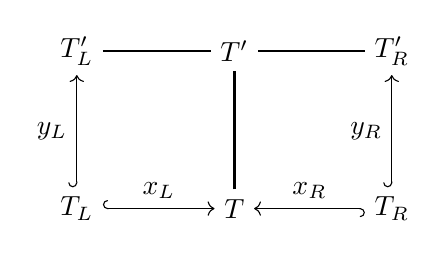
\begin{tikzpicture}
      \node (1) at (-2,1) {$T'_L$};
      \node (2) at (0,1) {$T'$};
      \node (3) at (2,1) {$T'_R$};
      \node (4) at (-2,-1) {$T_L$};
      \node (5) at (0,-1) {$T$};
      \node (6) at (2,-1) {$T_R$};
      \draw[right hook->] (4)--(5) node[midway,above] {$x_L$};
      \draw[right hook->] (6)--(5) node[midway,above] {$x_R$};
      \draw[right hook->] (4)--(1) node[midway,left] {$y_L$};
      \draw[right hook->] (6)--(3) node[midway,left] {$y_R$};
      \draw[thick] (1)--(2);
      \draw[thick] (3)--(2);
      \draw[very thick] (5)--(2);
    \end{tikzpicture}
    \caption{}
    \label{fig:DPjoinmap}
  \end{figure}

  Our first order of business is to rename all forgotten features in
  $T$ to their real features as given by $T_L'$ and $T_R'$. That is,
  for every node $t$ in $T$ assigned to a forgotten feature, i.e.,
  $\feat(t) \in \SoFF{[k_L]}\cup\SoFF{[k_R]}$, we do the following.
  If $\feat(t) \in \SoFF{[k_H]}$ for $H\in \{L,R\}$, then $t$ is also
  in $T_H$ and hence also in $T_H'$\note{todo: explain}. Therefore, we
  can change $\feat(t)$ to the real feature assigned to $t$ in
  $T_H'$. Let $T^0$ be the DT obtained from $T$ after renaming all
  forgotten features to real features in this manner.
  
  Consider an edge $e=(p,c)$ in $T_L$ such that $p$ is the parent of $c$
  in $T_L$. Then, $e$ corresponds to a path $P_L'(e)$ between
  $y_L(p)$ and $y_L(c)$ in $T_L'$. Similarily, $e$ corresponds to a
  path $P_L(e)$ between $x_L(p)$ and $x_L(c)$ in $T^0$.

  Our next order of business is now to add all nodes to $T^0$ that have been
  removed when going from $T_L'$ to $T_L$ (via the reduction
  $\red(\rel_{\rlstan{b_L}}(T_L'))$). To achieve this, we go over
  every edge $e=(p,c)$ of $T_L$ such that $p$ is the parent of $c$ in
  $T_L$ and plugin the path $P_L'(e)$ (from $T_L'$) into the last edge
  on the path $P_L(e)$ (from $T^0$). Let $T^1$ be the tree obtained from
  $T^0$ after doing this operation for every edge of $T_L$.
  
  % define the operation of pluging-in a path into an edge

  Consider an edge $e=(p,c)$ in $T_R$ such that $p$ is the parent of $c$
  in $T_R$. Then, $e$ corresponds to a path $P_R'(e)$ between
  $y_R(p)$ and $y_R(c)$ in $T_R'$. Similarily, $e$ corresponds to a
  path $P_R(e)$ between $x_R(p)$ and $x_R(c)$ in $T^1$. 
  Similarily to above, we now add all nodes to $T^1$ that have been
  removed when going from $T_R'$ to $T_R$ (via the reduction
  $\red(\rel_{\rlstan{b_R}}(T_R'))$). To achieve this, we go over
  every edge $e=(p,c)$ of $T_R$ such that $p$ is the parent of $c$ in
  $T_R$ and plugin the path $P_R'(e)$ (from $T_R'$) into the last edge
  on the path $P_R(e)$ (from $T^1$). Let $T'$ be the tree obtained from
  $T^1$ after doing this operation for every edge of $T_R$.

  We now show that $T'$ is indeed a witness for the validity of the record
  $(\hat{T},s_L+s_R)$, i.e., $T'$ is a reduced DT template for $b$
  such that
  $\hat{T}=\red(\rlstan{b}(T'))$ and $s_L+s_R=|V(T')\setminus V(\hat{T})|$.
  % continue here

  We start by showing that $\hat{T}=\red(\rel_{\rlstan{b}}(T'))$.
  Because $\hat{T}=\rlstan{b}(T^0)$, it suffices to show that the only
  nodes removed from $T'$ are the ones that we added to $T^0$ to
  obtain $T'$. Or in other words, we need to show that only the nodes
  that are redundant in $\rel_{\rlstan{b}}(T')$ are the nodes 
  in $V(T')\setminus V(T^0)$.

  % Consider a node $t \in V(T')\setminus V(\hat{T})$. Because $T'$ is
  % reduced and $t$ is redudant in $\rlstan{b}(T')$, we obtain that $t$
  % is assigned a real feature in $T'$, i.e., $\feat_{T'}(t) \in
  % \feat(b)$. Moreover, there must exists an ancestor $t'$ of $t$ in
  % $T'$ such that
  % $\rlstan{b}(\feat_{T'}(t))=\rlstan{b}(\feat_{T'}(t'))$, i.e., $t'$
  % is the reason why $t$ is redundant in $\rlstan{b}(T')$. 

  Consider a node $t \in
  V(T')\setminus V(T^0)$, i.e., $t$ is a node that we added to $T^0$
  to obtain $T'$. Then, $t \in V(T_H')\setminus V(T_H)$ for
  some $H \in \{L,B\}$. Because $T_H=\red(\rel_{\rlstan{b_H}}(T_H'))$,
  $t$ is redundant in $\rel_{\rlstan{b_H}}(T_H')$, because of some node
  $t' \in V(T_H)$ with
  $\rlstan{b_H}(\feat_{T_H'}(t))=\rlstan{b_H}(\feat_{T_H'}(t'))$.
  Since $t' \in
  V(T_H)$ also $t' \in V(T')$ and therefore $t$ is also redundant in 
  $\rel_{\rlstan{b}}(T')$ (because of $t'$), as required.

  Now consider a node $t \in V(T^0)$ and assume for a contradiction
  that $t$ is redundant in $\rlstan{b}(T')$ because of some node $t'
  \in V(T')$ with
  $\rlstan{b}(\feat_{T'}(t))=\rlstan{b}(\feat_{T'}(t'))$. Then,
  because $\hat{T}=\rlstan{b}(T^0)$ is reduced, we obtain that $t' \in
  V(T')\setminus V(T^0)$. Therefore, $t' \in V(T_H')\setminus V(T_H)$
  for some $H \in \{L,R\}$. But then, $t'$ is redundant in
  $\rel_{\rlstan{b}}(T_H')$ because of some node $t'' \in V(T_H)$ with
  $\rlstan{b}(\feat_{T'}(t''))=\rlstan{b}(\feat_{T_H'}(t'))$, which
  implies that also $t$ is redundant in $\hat{T}$ because of $t''$ a
  contradiction to our assumption that $\hat{T}$ is reduced. This
  shows that $\hat{T}=\red(\rel_{\rlstan{b}}(T'))$. Moreover, because
  $|V(T^0)|=|V(\hat{T})|$ and $|V(T')\setminus V(T^0)|=s_L+s_R$, it
  also follows that $s_L+s_R=|V(T')\setminus V(\hat{T})|$.
  \note{ proof of minimality of $T'$ is still missing}

  
  




  
  
  Moreover, $V(T)\setminus Im(x_H)$ and $V(T'_H)\setminus Im(y_H)$ can
  be partitioned into subtrees that have been deleted after the
  application of $r\circ p_*$, $r\circ p'_*$ on $T$ or of the standard
  reduction on $T'_H$: let $X^*_H$ and $Y^*_H$ be the set of roots of
  the above subtrees in $V(T)\setminus Im(x_H)$ and $V(T'_H)\setminus
  Im(y_H)$ respectively.
  In addition, for every element $y\in Y^*_H$, let $Y^H_y$ be the
  maximal subtree of $T'_H$ rooted at $y$ with no elements from
  $Im(y_H)$ and that does not contain any vertex from $Y^*_H\setminus
  \{y\}$; let $(Y^H_y,S^H_y)$ the corresponding single pair.
  In a similar way, for every element $x\in X^*_H$, let $X^H_x$ be the
  maximal subtree of $T$ rooted at $x$ with no elements from $Im(x_H)$
  and that does not contain any vertex from $X^*_H\setminus \{x\}$;
  let $(X^H_x,S^H_x)$ the corresponding single pair.
  Finally, for every $y\in Y^*_H$, let $P^H_y$ be the shortest
  downwards path in $T'_H$ that contains $y$ and with both endpoints
  in $Im(y_H)$, say $y_H(t)$ and $y_H(t')$.

\smallskip
\noindent
{\it Claim 1: For every $H\in \{L,R\}$ and for every $y,y'\in Y^*_H$, the paths $P^H_{y}$ and $P^H_{y'}$ are either edge disjoint or $P^H_{y}=P^H_{y'}$.}

\noindent
{\it Proof.} If $P^H_{y}$ and $P^H_{y'}$ are edge disjoint, then the statement is proven immediately. Suppose $P^H_{y}$ and $P^H_{y'}$ share an edge. By minimality and the fact they are downwards paths, $P^H_{y}$ and $P^H_{y'}$ share the endpoint towards the root. If they also share the other endpoint, then the statement is proven immediately. Suppose now their endpoints towards the leaves is different, say $w$ and $w'$, and consider the last edge those paths have in common in a root-to-leaf order, say $uv$. 

Without loss of generality, we can assume $w$ belongs to the left branch of $v$ and $w'$ belongs to the right branch of $v$. Note that $v\in V(T'_H)\setminus Im(y_H)$, or we get a contradiction due the minimality of $P^H_y$.
Now we get the following contradiction: by construction, $w$ and $w'$ are both elements of $Im(y_H)$ but at least one of them must be in $V(T'_H)\setminus Im(y_H)$ since it is an element of either $Y^H_{y}$ or of $Y^H_{y'}$. This proves Claim 1.

\smallskip
Now for every $y\in Y^*_H$ we consider the path $Q^H_y$ in $T$ having endpoints $x_H(t)$ and $x_H(t)$.

\smallskip
Now we are able to describe how to obtain a witness $T'$ of $T$ for $b$. 
For every $y\in Y^*_L$, in the last edge of path $Q^L_y$ we plug in the single pair $(Y^L_{y'},S^L_{y'})$ rooted at $y'$, for every internal node $y'$ of $P^L_y$, in the order the nodes $y'$ apprear in $P^L_y$. Note that, in the case an element of $Y^*_L$ is present in more than one $P^L_y$, we plug in the corresponding single pair only once. Note also that whenever we plug in some single pair $(Y^L_{y},S^L_{y})$ in a DT, the tree $Y^L_{y}$ has real features and future features as nodes. Call this graph $T^*$. Now we do the same sequence of plug ins of the single pairs corresponding to the internal vertices of $P^R_y$ in the last edge of the path $Q^R_y$. Again, in the case an element of $Y^*_R$ is present in more than one $P^R_y$, we plug in the corresponding single pair only once. Call the tree obtained in this way $T'$. Node that $T'$ contains real features from $feat(b_L)$ and from $feat(b_R)$ and future features with labels in $\mathcal{P}([k])$.

\smallskip
To conclude this part of the proof we have to show two things: $(i)$ $T$ is obtained from $T'$ after removing $s$ vertices; $(ii)$ $T'$ is a real DT for $b$. We start proving $(i)$: by construction $T'$ is obtained from $T$ after adding $s_L$ elements from $T'_L$ and $s_R$ elements from $T'_R$, and so with $s_L+s_R=s$ more elements. 

Before considering statement $(ii)$, we consider the following relabelling $p_+$ of $T'$: every real feature in $feat(b_R)$ is a assigned to a feature with its label at node $b_R$ and every other feature is assigned to itself. The real DT $T'_L$ can be obtained from $T'$ by the application of the composition $r \circ p_* \circ p_+$.

Now we consider statement $(ii)$. We show that given an example $e\in exam(b_L)$, $e$ is correctly classified by $T'$ and to do so we show that $e$ ends in a leaf of $T'$ that corresponds to the leaf where $e$ ends in $T'_L$. 
Say that $e$ goes along a path $P$ of $T'_L$ from the root to a leaf $\ell$ and let $Q$ be the corresponding path in $T'$, i.e. the path from $r$ to $\ell$ (note that by construction $\ell$ is present in $T'$ and is still a leaf). 
Let $v$ be a node of $Q$, we can have the following different cases.

\begin{itemize}
\item $v$ is a real feature from $feat(b_L)$: $v$ is also present in $T'_L$ as real feature; 
\item $v$ is a real feature from $feat(b_R)$: $v$ might not be present in $T'_L$ due reductions but if it is present it is a future feature $A_i$ for some $i\in [k]$;
\item $v$ is a future feature $f_A$: $v$ might not be present in $T'_L$ due reductions but if it is present it is still the same future feature $A_i$.
\end{itemize}

If $v$ is present in $T'_L$ then the behaviour of $v$ on $e$ in $T'_L$ and in $T'$ is the same. Suppose now $v$ is a node of $Q$ that is being reduced due his label and so it is not present in $T'_L$. This means there is a set of ancestors of $v$ such that their labels allows to remove $v$ and by construction $v$ behaves on $e$ like those ancestors. This proves $e$ goes along $Q$ and in particular it ends at leaf $\ell$ and so $T'$ is a real DT for $b_L$. With symmetric construction, we show that $T'$ is also a real DT for $b_R$.

\medskip
Now we prove the backward direction. Let $T$ be a reduced DT such that $s$ is the minimum number of elements that have been deleted from a witness $T'$ of $T$ for $b$. In particular, we recall that $T'$ is a real DT for $b$ with actual feature labels in $[k]\cup [k']$ and future feature labels in $\mathcal{P}([k])$. 

We create at real DT $T'_L$ by the application of the composition $r \circ p_* \circ p_+$ to $T'$. By assumption $T'$ is a real DT for $b_L$ and by construction $T'_L$ is a real DT for $b_L$. 
Denote with $T_L$ the DT template obtained from $T'_L$ by standard reduction and denote with $s_L$ the number of nodes that have been deleted from $T'_L$ to obtain $T$. By induction we have $(T_L,s_L)\in \mathcal{R}(b_L)$.
Now we note that $T_L$ is obtained from $T$ after the application of the composition $r \circ p_*$. In a symmetric way, we construct $T'_R$, $T_R$ and the record $(T_R,s_R)\in \mathcal{R}(b_R)$. Then $(T,s_L+s_R)\in \mathcal{R}(b)$.
\end{proof}

<<<<<<< HEAD
\begin{lemma}[relabel node]\label{lem:relabel}
Let $b\in V(B)$ be relabel node. Then $\mathcal{R}(b)$ can be computed in time $\mathcal{O}(k(2k+2^k+2)2^{3k+1})$.
\end{lemma}

\begin{proof}
Let $b_C$ be the unique child of $b$ in $B$. Let $R$ be the mapping of $[k]$ to itself that represent the node $b$. Moreover, since we are considering a {\it nice} NLC-expression we can assume $R$ is the identity mapping, i.e. $R(\ell)=\ell$, for all values except for a unique element $i$ of its domain, i.e. $R(i)=j$ for some $j\in [k]\setminus \{i\}$.

We say that a future feature $A$ is {\it good} if it does not distinguish between $i$ and $j$, that is $i\in A$ if and only if $j\in A$, and {\it bad} otherwise. Let $(T_C,s_C)$ be an element of $\mathcal{R}(b_C)$. Let $p''$ the following relabelling of the DT template $T_C$: every feature with label $i$ is assigned to label $j$ and every future feature with label $A$ is assigned to the future feature with label $A\setminus \{i\}$. 

If $T_C$ has a bad future feature then we do not take any other action. Suppose now $T_C$ has only good future features; now let $T$ be the DT template obtained from $T_C$ after the application of the composition $r \circ p''$ and let $s^*$ be the number of nodes that have been deleted from $T_C$ to $T$.

If there is a record in $\mathcal{R}(b)$ of the form $(T,s')$ for some integer $s'\leq s_C+s^*$ then we do not take any other action.
If there is a record in $\mathcal{R}(b)$ of the form $(T,s')$ for some integer $s'>s_C+s^*$ then we replace it with $(T,s_C+s^*)$.
If there is no record in $\mathcal{R}(b)$ of the form $(T,s')$ for some integer $s'$ then we add $(T,s_C+s^*)$ to $\mathcal{R}(b)$.

\medskip
Now we want to evaluate the running time of computing $\mathcal{R}(b)$. Consider record $(T_C,s_C)$ in $\mathcal{R}(b_C)$. In $\mathcal{O}(k)$ time we check if $T_C$ all the future features are good. For every such DT $T_C$, there are at most $2^{2k}$ paths from the root to the leaves and for every of these paths there are at most $k$ nodes for each of the following: feature with label $i$ and and future feature that contains $i$. This means $r \circ p''$ can be done in $\mathcal{O}(k)$ time.
%GP: $r$ can be done together with $p''$ as we can relabel nodes top-to-bottom and check at the same time if it can be reduce.
This means to compute $\mathcal{R}(b)$ takes $\mathcal{O}(k|\mathcal{R}(b_C)|)=\mathcal{O}(k(2k+2^k+2)2^{3k+1})$ time.

\medskip
Now we have to show the correctness of the construction for $\mathcal{R}(b)$, i.e. $(T,s)\in \mathcal{R}(b)$ if and only if $s$ is the minimum number of elements that have been deleted from a witness $T'$ of $T$ for $b$.

\smallskip
We start with the forward direction. Let $(T,s)\in \mathcal{R}(b)$. By construction there exists a record $(T_C,s_C)\in \mathcal{R}(b_C)$ such that $T$ is obtained from $T_C$ after the application of $r \circ p''$ and let $s^*=s-s_C$. By induction $s_C$ is the minimum amount of nodes that have been deleted from a witness $T'_C$ of $T_C$ for $b_C$. By construction we also know that every future feature of both $T'_C$ and $T_C$ is good.

Denote with $T'$ the real DT obtained $T'_C$ after the application of $r \circ p''$: note that this last reduction does not any node since every future feature of $T'_C$ is good and there is no feature with label $i$. To conclude this part of the proof we have to show two things: $(i)$ $T$ is obtained from $T'$ after removing $s$ vertices; $(ii)$ $T'$ is a witness of $T$ for $b$. 

Before proving $(i)$, we describe how $T$ can be obtained from $T'$. Let $p'''$ be the following relabelling of $T'$: every real feature that contains $j$ is assigned to the real feature $A\cup \{i\}$ and every other feature is assigned to itself. Then the application of the composition $p'''$, the standard reduction and $r \circ p''$ to $T'$ is exactly the standard reduction for $T'$ which then result to the DT template $T$.
By Lemma~\ref{red-last} the score of the standard reduction from $T'$ to $T$ is exactly $s_C+s^*=s$. 

Now we consider statement $(ii)$. First note that $exam(b)=exam(b_C)$.
We show that a given example $e\in exam(b)$ is correctly classified by $T'$. Say that $e$ goes along a path $P$ of $T'_C$ from the root to a leaf $\ell$. We show $e$ goes along the path $P$ in $T'$ as well: every real feature has not changed and so $e$ behaves the same. Since every future feature of $T'_C$ is good, then $e$ behave the same on the corresponding future feature of $T'$.

\smallskip
Now we prove the backward direction. Let $T$ be a reduced DT such that $s$ is the minimum number of elements that have been deleted from a witness $T'$ of $B$ for $b$. In particular, we recall that real $T'$ is a DT for $b$ with real features and future feature labels in $\mathcal{P}([k]\setminus \{i\})$.

We create the real DT $T'_C$ as the application of $r \circ p'''$ to $T'$, the DT template $T_C$ as the application of the standard reduction to $T'_C$. By construction we have $(T_C,s_C)\in \mathcal{R}(b_C)$, where $s_C$ is the number of nodes that have been removed from $T'_C$ to $T_C$. Note that $T_C$ has only good future features.
Finally we note that $T$ is obtained from $T_C$ by the application of $r \circ p''$.
\end{proof}

\subsection{Formal Definition of Records and Preliminary Results}

=======
\newpage
\section*{NLC-width}
>>>>>>> e150fdde332112fd1c2acb6bd85a9a5606b79547
We start off with some definitions. We say an edge is a {\it left (right) edge} of a subcubic rooted tree if it connects a non-leaf node with his left (resp. right) child. Let $Y$ be a rooted subcubic tree and $S\in \{left,right\}$, then we say the pair $(Y,S)$ is a {\it single pair} if the root of $Y$ has at most one child and the side $S$ indicates whether the edge from the root is either a left or right edge. Moreover, we say that $(Y,S)$ is single pair in a subcubic rooted tree $T$ if $Y$ is a maximal subtree of $T$ and in $Y$ the root have at most the $S$ child. Note that when tree of a single pair is made of just a node, the side is not relevant.

Now we can define two operations on subcubic rooted trees and single pairs. We say that we {\it plug in} a single pair $(Y,S)$ in a left (right) edge $uv$ as follows: we make the root $y$ of $Y$ the left (right) child of $u$, $Y\setminus \{y\}$ to be the $S$ subtree of $y$ and $v$ to be the $H\in \{left,right\}\setminus S$ child of $y$. See Figure~\ref{fig:plugin} for the corresponding drawings. Note after a plug in of a single pair in an edge, the node $v$ belongs in the same side of the subtree rooted at $u$ as it was before the plug in.

\begin{figure}[h]
\begin{minipage}{0.2\textwidth}
\centering
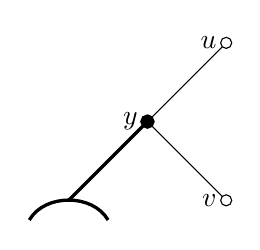
\begin{tikzpicture}[scale=1]
\draw (0,1)--(-1,-0)--(0,-1);
\draw[fill=white] (0,1) circle [radius=2pt]
(0,-1) circle [radius=2pt];
\draw[very thick,fill=black] (-1,0) circle [radius=2pt] (-1,0)--(-2,-1);
\draw[very thick] (-2.5,-1.25) to[out=60,in=120] (-1.5,-1.25);
\node[left] at (0,1) {$u$};
\node[left] at (-1,0) {$y$};
\node[left] at (0,-1) {$v$};
\end{tikzpicture}
\subcaption{$(Y,left)$~left.}
\end{minipage}
\begin{minipage}{0.2\textwidth}
\centering
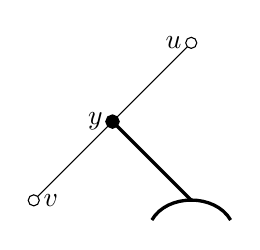
\begin{tikzpicture}[scale=1]
\draw (0,1)--(-2,-1);
\draw[fill=white] (0,1) circle [radius=2pt]
(-2,-1) circle [radius=2pt];
\draw[very thick,fill=black] (-1,0) circle [radius=2pt] (-1,0)--(0,-1);
\draw[very thick] (-0.5,-1.25) to[out=60,in=120] (0.5,-1.25);
\node[left] at (0,1) {$u$};
\node[left] at (-1,0) {$y$};
\node[right] at (-2,-1) {$v$};
\end{tikzpicture}
\subcaption{$(Y,right)$~left.}
\end{minipage}
\begin{minipage}{0.25\textwidth}
\centering
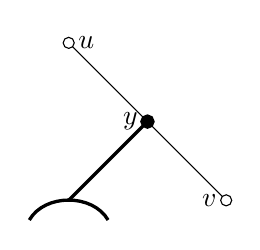
\begin{tikzpicture}[scale=1]
\draw (-2,1)--(0,-1);
\draw[fill=white] (-2,1) circle [radius=2pt]
(0,-1) circle [radius=2pt];
\draw[very thick,fill=black] (-1,0) circle [radius=2pt] (-1,0)--(-2,-1);
\draw[very thick] (-2.5,-1.25) to[out=60,in=120] (-1.5,-1.25);
\node[right] at (-2,1) {$u$};
\node[left] at (-1,0) {$y$};
\node[left] at (0,-1) {$v$};
\end{tikzpicture}
\subcaption{$(Y,left)$~right.}
\end{minipage}
\begin{minipage}{0.2\textwidth}
\centering
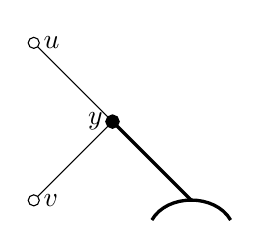
\begin{tikzpicture}[scale=1]
\draw (-2,1)--(-1,0)--(-2,-1);
\draw[fill=white] (-2,1) circle [radius=2pt]
(-2,-1) circle [radius=2pt];
\draw[very thick,fill=black] (-1,0) circle [radius=2pt] (-1,0)--(0,-1);
\draw[very thick] (-0.5,-1.25) to[out=60,in=120] (0.5,-1.25);
\node[right] at (-2,1) {$u$};
\node[left] at (-1,0) {$y$};
\node[right] at (-2,-1) {$v$};
\end{tikzpicture}
\subcaption{$(Y,right)$~right.}
\end{minipage}
\caption{The drawings describe the plug in operation in the different four cases. The bold part highlight the single pair $(Y,S)$.}
\label{fig:plugin}
\end{figure}

Let $(Y,S)$ be a single pair in a rooted subcubic tree $T$, then we {\it remove} $(Y,S)$ from $T$ as follows. Let $y$ be the root of $Y$. If $y$ is the root of $T$, then we obtain an empty tree. If $y$ is a leaf node of $T$, then we obtain $T-y$. Otherwise let $y$ be a non-root and non-leaf node, let $u$ be the parent of $y$ and $v$ be the child of $y$ that is not in $V(Y)$, then we consider the tree obtained from $T$ after replacing $y$ with $v$ as the child of $u$ and deleting $Y$. See Figure~\ref{fig:reduction} for an example.

\begin{figure}[h]
\begin{minipage}{0.5\textwidth}
\centering
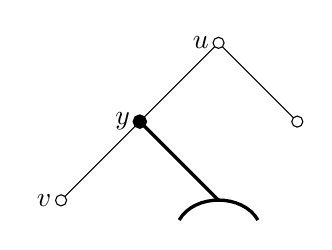
\begin{tikzpicture}[scale=1]
\draw (0,1)--(-2,-1) (0,1)--(1,0);
\draw[fill=white] (0,1) circle [radius=2pt]
(1,0) circle [radius=2pt]
(-2,-1) circle [radius=2pt];
\draw[very thick,fill=black] (-1,0) circle [radius=2pt] (-1,0)--(0,-1);
\draw[very thick] (-0.5,-1.25) to[out=60,in=120] (0.5,-1.25);
\node[left] at (0,1) {$u$};
\node[left] at (-1,0) {$y$};
\node[left] at (-2,-1) {$v$};
\end{tikzpicture}
\end{minipage}
\begin{minipage}{0.1\textwidth}
\centering
\begin{tikzpicture}[scale=1]
\draw (0,1)--(-2,-1) (0,1)--(1,0);
\draw[fill=white] (0,1) circle [radius=2pt]
(1,0) circle [radius=2pt]
(-2,-1) circle [radius=2pt];
\node[left] at (0,1) {$u$};
\node[left] at (-2,-1) {$v$};;
\end{tikzpicture}
\end{minipage}
\caption{The drawing describe an example of the remove operation: a single pair $(Y,right)$ is removed from a subcubic rooted tree. The bold part highlight the single pair $(Y,S)$.}\label{fig:reduction}
\end{figure}

It is clear from the four different plug in cases that if we want to plug in two pairs $(Y,S)$ and $(Y',S')$ on an edge $uv$ such that the ancestor-descendant relationship is given, say $y$ of $Y$ has to be in the path from the root to $y'$ of $Y'$, then we can do these plug ins in any order but with some care. It is the same if we first plug in $(Y,S)$ in the edge $uv$ and then plug in $(Y',S')$ in the edge $yv$ or if we first plug in $(Y',S')$ in the edge $uv$ and then plug in $(Y,S)$ in the edge $uy'$. See Figure~\ref{fig:multiplugin} for the an example.

\begin{figure}[h]
\centering
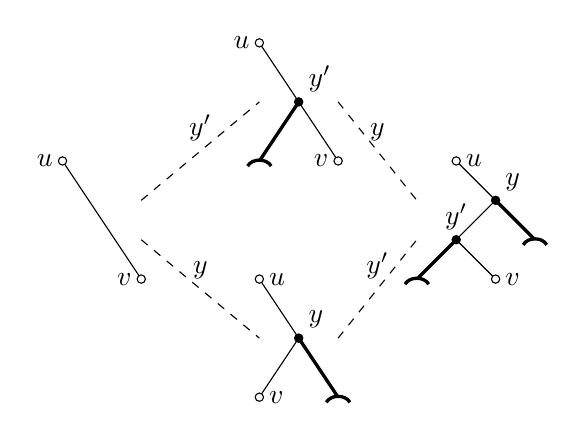
\begin{tikzpicture}[scale=0.5]
\draw[dashed] (-5,0)--(-2,2.5) node[midway,above] {$y'$}
(-5,-1)--(-2,-3.5) node[midway,above] {$y$}
(0,2.5)--(2,0) node[midway,above] {$y$}
(0,-3.5)--(2,-1) node[midway,above] {$y'$};
\draw (-7,1)--(-5,-2) (-2,4)--(0,1) (-2,-2)--(-1,-3.5)--(-2,-5) (3,1)--(4,0)--(3,-1)--(4,-2);
\draw[very thick] (-1,-3.5)--(0,-5) (-1,2.5)--(-2,1) (4,0)--(5,-1) (3,-1)--(2,-2) (-2.3,0.87) to[out=60,in=120] (-1.7,0.87)
(-0.3,-5.13) to[out=60,in=120] (0.3,-5.13) (4.7,-1.13) to[out=60,in=120] (5.3,-1.13) (1.7,-2.13) to[out=60,in=120] (2.3,-2.13);
\draw[fill=white] (-7,1) circle [radius=3pt] (-5,-2) circle [radius=3pt] (-2,4) circle [radius=3pt] (0,1) circle [radius=3pt] (-2,-2) circle [radius=3pt] (-2,-5) circle [radius=3pt] (3,1) circle [radius=3pt] (4,-2) circle [radius=3pt];
\draw[fill=black] (-1,-3.5) circle [radius=3pt] (-1,2.5) circle [radius=3pt] (4,0) circle [radius=3pt] (3,-1) circle [radius=3pt];
\node[left] at (-7,1) {$u$};
\node[left] at (-2,4) {$u$};
\node[right] at (-2,-2) {$u$};
\node[right] at (3,1) {$u$};
\node[left] at (-5,-2) {$v$};
\node[left] at (0,1) {$v$};
\node[right] at (-2,-5) {$v$};
\node[right] at (4,-2) {$v$};
\node[above right] at (4,0) {$y$};
\node[above right] at (-1,-3.5) {$y$};
\node[above right] at (-1,2.5) {$y'$};
\node[above] at (3,-1) {$y'$};
\end{tikzpicture}
\caption{An example of plugging in two pairs $(Y,left)$ and $(Y',right)$ in a left edge $uv$.}
\label{fig:multiplugin}
\end{figure}

For a subset of labels $A\subseteq [k]$, we define the feature template $f_A$ by setting $e(f_A)=1$ if and only if $lab(e)\in A$ and $e(f_A)=0$ otherwise. With a small abuse of notation, we often identify the feature template $f_A$ with the corresponding subset of labels $A$.

\smallskip
Suppose we have a DT such that some feature label~$i$ occurs twice on a path from the root to the leaves, say~$f_1$ is the instance closer to the root and~$f_2$ is the other instance. If~$f_2$ is in the left (resp. right) subtree of~$f_1$, we remove $f_2$'s right (resp. left) subtree. In this case we say we have done an {\it actual removal}.

Suppose we have a feature template labelled~$A$ in our decision tree. Let $A_1,\ldots,A_\ell$ be the sequence of feature templates on the path from the root to~$A$ in order (not including~$A$). Let $A_i'=A_i$ if~$A$ is in the right sub-tree of~$A_i$ and let $A_i'=\overline{A_i}$ otherwise. If $\overline{A} \subseteq A_1' \cup \ldots \cup A_\ell'$, then we remove the subtree rooted at the left child of~$A$. If $A\subseteq \overline{A_1'} \cup \ldots \cup \overline{A_\ell'}$, then we remove the subtree rooted at the right child of~$A$. In this case we say we have done a {\it template removal}. If this procedure has been applied to a record exhaustively, we say that the DT is {\it reduced}.

To be short, for a DT $T$ and a node $v$, we write $v\in T$ instead of $v\in V(T)$ and $v\not\in T$ otherwise. In a DT $T$ we say that path $p$ is a {\it downward} pard path if it is contained in a path having the root as endpoint.

We now formally define two important operations. Given a DT $T$, we say that we {\it reduce} $T$ if we exhaustively do actual removals and template removals. Call $r(T)$ the resulting DT.

Recall that in any DT $T$, every non-leaf node $v$ has one of the following three contents: $v$ is a real feature (without label), or $v$ is a feature with a label, or $v$ is a future feature with the corresponding subset of labels.
A {\it relabelling} $p$ for $T$ is an assignment of contents of $T$ as follows. Every feature is assigned to a feature with is either future, real or with a label. We say that we {\it relabel} the DT $T$ via the relabelling $p$ if for every node of $T$ we apply the corresponding assignment and call $p(T)$ the resulting DT.

The following lemma shows that, after repeatedly applying it the necessary amount of times, to obtain a reduced DT after a sequence of relabels, it is safe to reduce at the end.

\begin{lemma}[Relabelling Lemma]\label{red-last}
Let $T$ be a DT and $p$ be relabelling of $T$. Then $(r \circ p \circ r) (T)=(r \circ p) (T)$.
\end{lemma}

\begin{proof}
For every $v\in T$, we want to prove $v\in (r\circ p\circ r)(T) \Leftrightarrow v\in (r \circ p)(T)$.

$\Rightarrow$ Suppose there is a node $v\not\in (r \circ p)(T)$. Since $v\in p(T)$, there is a set of ancestors of $v$ in $p(T)$ that allows to remove $v$. Let $A_v$ be the union of all the minimal set of ancestors of $v$ in $p(T)$ that allows to remove $v$. If $A_v$ is a set of ancestors of $v$ in $T$ that allows to reduce $v$ then $v\not\in r(T)$ and so $v\not \in (r\circ p\circ r)(T)$. Otherwise let $A'_v$ be the subset of $A_v$ in $(p \circ r)(T)$. We conclude by noting that $A'_v$ contains one of the minimal sets $A_v$ is composed of and so $v\not \in (r\circ p\circ r)(T)$.

$\Leftarrow$ Suppose there is a node $v\not\in (r \circ p \circ r)(T)$. If $v\in (p \circ r)(T)$, there exists a set $A_v$ of ancestors of $v$ in $(p \circ r)(T)$ that allows to reduce $v$. Then $A_v$ is a set of ancestors of $v$ in $p(T)$ that allows to reduce $v$ and so $v\not\in (r \circ p)(T)$. If $v\not\in (p \circ r)(T)$ then $v\not\in r(T)$: there exists a set $A_v$ of ancestors of $v$ in $T$ that allows to remove $v$. This means $A_v$ is a set of ancestors of $v$ in $p(T)$ that allows to remove $v$ and so $v\not\in (r \circ p)(T)$.
\end{proof}

We say that a DT $T$ is a {\it real DT} if every non-leaf node is either a real feature or a future feature, whereas it is a {\it DT template} if it contains no real feature.

Let $B$ be a rooted subcubic tree that corresponds to a $k$-NLC expression of the graph $G_I(E)$.
For $b\in V(B)$, we write $feat(b)$ and $exam(b)$ for the sets of features and examples introduced at nobe $b$.
We say that a real DT $T$ is a DT for the node $b$ if every real feature of $T$ is an element of $feat(b)$ and every example in $exam(b)$ is correctly classified by $T$, i.e. if $e\in exam(b)\cap E^+$ then $e$ ends in a leaf with a $+$ label and if $e\in exam(b)\cap E^-$ then $e$ ends in a leaf with a $-$ label.

Given a real DT $T$ and a node $b\in B$, often we want to perform a very specific composition of operations. Let $p_b$ be the following relabelling of $T$: every real feature of $T$ is assigned to a feature with the label given by the $k$-NLC expression at node $b$ and every other feature is assigned to itself. Then the composition $r \circ p_b$ is called the {\it standard reduction} of $T$ at node $b$.
Given a DT $T$ and a node $b\in B$, it is useful to give the following relabelling $p'_b$: every feature with a label is assigned to the real feature of that node. The relabelling $p'_b$ is called the {\it real relabelling} of $T$ at node $b$.

We say that a DT template $T$ is a DT for the node $b$ if there exits a real DT $T'$ for $b$ such that $T$ is the standard reduction of $T'$. In this case we say that $T'$ is the witness of $T$ for $b$.

\begin{lemma}\label{lem:reduced-tree-height}
If there are $\ell$ features with labels and $2^h$ future features, then every reduced DT template has height at most~$\ell+h$. Furthermore, every path from the root to the leaves contains at most~$\ell$ features with label and at most $h-1$ future features.
\end{lemma}

\begin{proof}
Consider a path~$P$ of maximum length from the root to the leaves in a reduced DT template $T$. 
By the assumptions on $T$, no feature with label appears more than once on this path: the number of these feature nodes on this path is at most~$\ell$. Consider two future features $f_{A}$ and $f_{A'}$ that appear in $P$, say $f_{A}$ is the instance closer to the root. Since $T$ is reduced, we must have that $\emptyset\subset A'\subset A$. Since the label of any future feature has at most $h$ elements, there can be at most $h-1$ feature template nodes on this path. The path ends with a leaf node, so this gives a total of $\ell+h-1+1=\ell+h$ nodes, as required.
\end{proof}

\begin{lemma}\label{lem:reduced-tree-number}
If there are $\ell$ features with label and $2^h$ future features, 
then there are at most $(\ell+2^k+2)2^{\ell+k+1}$ reduced DT templates. Furthermore, these can be enumerated in $\mathcal{O}((\ell+2^k+2)2^{\ell+k+1})$-time.
\end{lemma}

\begin{proof}
By Lemma~\ref{lem:reduced-tree-height}, the tree has height at most $\ell+k$.
Each node of the decision tree could be a feature with label, a future feature, or a leaf: at most $\ell+2^h+2$ different contents. Since there are at most $2^{\ell+h+1}$ nodes in the tree, there are at most $(\ell+2^h+2) 2^{\ell+h+1}$ possible decision trees.
\end{proof}

\smallskip
The {\it semantics} for a record are defined as follows. We say that a pair $(T,s)$ is a {\it record} for the node $b\in B$ and we write $(T,s)\in \mathcal{R}(b)$, if $T$ is a DT template for $b$ and $s$ is the minimum number of elements that have been deleted from a witness $T'$ of $T$ for $b$.

\subsection{Proof to the Main Result}

Now, it suffices to compute $\mathcal{R}(b)$ via leaf-to-root dynamic programming. The following four lemmas show how this can be achieved for all of the four types of nodes in a $k$-NLC expression tree $B$.

\begin{lemma}[leaf node]\label{lem:leaf}
Let $b\in V(B)$ be a leaf node. Then $\mathcal{R}(b)$ can be computed in time $\mathcal{O}(k(2^k+3)2^{k+2})$.
\end{lemma}

\begin{proof}
Let $v$ be the vertex of $G_I(E)$ that corresponds to the leaf node $b$. This means either $v\in E$ or $v\in feat(E)$.

We have to enumerate all possible reduced DT templates $T$ for $b$. It is enough to consider all reduced DT templates $T$ of height at most $k+1$ and discard those that are not DT templates for $b$; these can be enumerated in time $\mathcal{O}((2^k+3)2^{k+2})$ by Lemma~\ref{lem:reduced-tree-number} and the check can be done in time $\mathcal{O}(k)$. We add the pair $(T,0)$ to the set of records $\mathcal{R}(b)$. 

Now we have to show the correctness of the construction for $\mathcal{R}(b)$, i.e. $(T,s)\in \mathcal{R}(b)$ if and only if $s$ is the minimum number of elements that have been deleted from a witness $T'$ of $T$ for $b$.

We start with the forward direction. Let $(T,s)\in \mathcal{R}(b)$. By construction, we have that $s=0$ and $T$ is a DT template for $b$ which is already reduced. Then $T$ is trivially a witness of $T$ for $b$.

Now we prove the backward direction. Let $T$ be a reduced DT template such that $0$ is the minimum number of elements that have been deleted from a witness $T'$ of $T$ for $b$. This means $T'$ is obtained from $T$ after the real relabelling at node $b$ is applied: $T$ is a DT template among the considered DTs above which leads to the fact that $(T,0)\in \mathcal{R}(b)$.
\end{proof}

\begin{lemma}[join node]\label{lem:join}
Let $b\in V(B)$ be a join node. Then $\mathcal{R}(b)$ can be computed in time $\mathcal{O}(k(2k+2^k+2)2^{6k+1})$.
\end{lemma}

\begin{proof}
Let $b_L$ and $b_R$ be the left, resp. right, child of $b$ in $B$: we may assume the labels for $feat(b_L)$ are in $[k]$ and the labels for $feat(b_R)$ are in $[k']$. Moreover, let $M$ be the $k\times k$ $\{0,1\}$ matrix that represent the node $b$. Finally, for every label $i\in [k]$, let $A_i=\{j\in [k]~|~M_{i,j}=1\}$.

We consider every reduced DT $T$ for $b$ with feature labels in $[k]\cup [k']$ and future feature labels in $\mathcal{P}([k])$; these can be enumerated in time $\mathcal{O}((2k+2^k+2)2^{3k+1})$ by Lemma~\ref{lem:reduced-tree-number}.

For every such DT $T$, we create a DT $T_L$ as follows. Let $p_*$ be the following relabelling: for every $i'\in [k']$, every feature with label $i'$ is assigned to the future feature $A_i$. Then we apply the composition $r \circ p_*$ to $T$. In a symmetrical way we create a DT $T_R$. Let $p'_*$ be the following relabelling: for every $i\in [k]$, every feature with label $i$ is assigned to the future feature $A_{i'}$ and every future feature $A_i$ is assigned to the future feature $A_{i'}$. Then we apply the composition $r \circ p'_*$ to $T$.

Now we want to understand if there is a record in $\mathcal{R}(b_L)$ of the form $(T_L,s_L)$ for some positive integer $s_L$ and if there is a record in $\mathcal{R}(b_R)$ of the form $(T_R,s_R)$ for some positive integer $s_R$: if the answer is yes in both cases, we add a record $(T,s_L+s_R)$ to $\mathcal{R}(b)$; otherwise we discard this option.

\medskip
Now we want to evaluate the running time of computing $\mathcal{R}(b)$. Every reduced DT $T$ can be enumerated in time $\mathcal{O}((2k+2^k+2)2^{3k+1})$ by Lemma~\ref{lem:reduced-tree-number}.
For every such DT $T$, there are at most $2^{3k}$ paths from the root to the leaves and for every of these paths there are at most $k$ nodes for each of the following: features with label in $[k]$, features with label in $[k']$ and future features by Lemma~\ref{lem:reduced-tree-height}.
This means $r \circ p_*$ and $r \circ p'_*$ can be done in $\mathcal{O}(k2^{3k})$ time.
%GP: $r$ can be done together with $p_*$ as we can relabel nodes top-to-bottom and check at the same time if it can be reducde.

\medskip
Now we have to show the correctness of the construction for $\mathcal{R}(b)$. We start with the forward direction. Let $(T,s)\in \mathcal{R}(b)$. By construction there exist records $(T_L,s_L)\in \mathcal{R}(b_L)$ and $(T_R,s_R)\in \mathcal{R}(b_R)$ such that $T_L$ and $T_R$ are obtained by the application of $r \circ p_*$ and $r \circ p'_*$ respectively to $T$ and $s_L+s_R=s$.

By induction, for $H\in \{L,R\}$, we know that $s_H$ is the minimum number of elements that have been deleted from a witness $T'_H$ of $T_H$ for $b_H$.

For $H\in \{L,R\}$, we define maps $x_H$ and $y_H$ as follows. Let $x_H~:~V(T_H)\to V(T)$ and $y_H~:~V(T_H)\to V(T'_L)$ be the functions that maps every node of $T_H$ to the corresponding node in $T$ and in $T'_L$ and note that by constructions both these maps are injective. 

\begin{figure}[h]
\centering
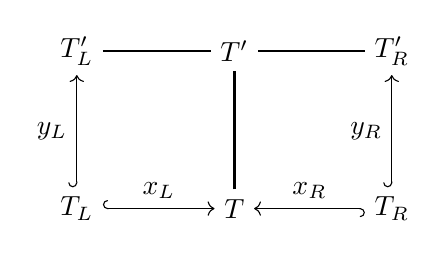
\begin{tikzpicture}
\node (1) at (-2,1) {$T'_L$};
\node (2) at (0,1) {$T'$};
\node (3) at (2,1) {$T'_R$};
\node (4) at (-2,-1) {$T_L$};
\node (5) at (0,-1) {$T$};
\node (6) at (2,-1) {$T_R$};
\draw[right hook->] (4)--(5) node[midway,above] {$x_L$};
\draw[right hook->] (6)--(5) node[midway,above] {$x_R$};
\draw[right hook->] (4)--(1) node[midway,left] {$y_L$};
\draw[right hook->] (6)--(3) node[midway,left] {$y_R$};
\draw[thick] (1)--(2);
\draw[thick] (3)--(2);
\draw[very thick] (5)--(2);
\end{tikzpicture}
\end{figure}

Moreover, $V(T)\setminus Im(x_H)$ and $V(T'_H)\setminus Im(y_H)$ can be partitioned into subtrees that have been deleted after the application of $r\circ p_*$, $r\circ p'_*$ on $T$ or of the standard reduction on $T'_H$: let $X^*_H$ and $Y^*_H$ be the set of roots of the above subtrees in $V(T)\setminus Im(x_H)$ and $V(T'_H)\setminus Im(y_H)$ respectively.  
In addition, for every element $y\in Y^*_H$, let $Y^H_y$ be the maximal subtree of $T'_H$ rooted at $y$ with no elements from $Im(y_H)$ and that does not contain any vertex from $Y^*_H\setminus \{y\}$; let $(Y^H_y,S^H_y)$ the corresponding single pair.
<<<<<<< HEAD
=======
%GP: add figure
>>>>>>> e150fdde332112fd1c2acb6bd85a9a5606b79547
In a similar way, for every element $x\in X^*_H$, let $X^H_x$ be the maximal subtree of $T$ rooted at $x$ with no elements from $Im(x_H)$ and that does not contain any vertex from $X^*_H\setminus \{x\}$; let $(X^H_x,S^H_x)$ the corresponding single pair. 
Finally, for every $y\in Y^*_H$, let $P^H_y$ be the shortest downwards path in $T'_H$ that contains $y$ and with both endpoints in $Im(y_H)$, say $y_H(t)$ and $y_H(t')$. 

\smallskip
\noindent
{\it Claim 1: For every $H\in \{L,R\}$ and for every $y,y'\in Y^*_H$, the paths $P^H_{y}$ and $P^H_{y'}$ are either edge disjoint or $P^H_{y}=P^H_{y'}$.}

\noindent
{\it Proof.} If $P^H_{y}$ and $P^H_{y'}$ are edge disjoint, then the statement is proven immediately. Suppose $P^H_{y}$ and $P^H_{y'}$ share an edge. By minimality and the fact they are downwards paths, $P^H_{y}$ and $P^H_{y'}$ share the endpoint towards the root. If they also share the other endpoint, then the statement is proven immediately. Suppose now their endpoints towards the leaves is different, say $w$ and $w'$, and consider the last edge those paths have in common in a root-to-leaf order, say $uv$. 

Without loss of generality, we can assume $w$ belongs to the left branch of $v$ and $w'$ belongs to the right branch of $v$. Note that $v\in V(T'_H)\setminus Im(y_H)$, or we get a contradiction due the minimality of $P^H_y$.
Now we get the following contradiction: by construction, $w$ and $w'$ are both elements of $Im(y_H)$ but at least one of them must be in $V(T'_H)\setminus Im(y_H)$ since it is an element of either $Y^H_{y}$ or of $Y^H_{y'}$. This proves Claim 1.

\smallskip
Now for every $y\in Y^*_H$ we consider the path $Q^H_y$ in $T$ having endpoints $x_H(t)$ and $x_H(t)$.

\smallskip
<<<<<<< HEAD
=======
\noindent
{\it Claim 2: For every $H\in \{L,R\}$ and for every $y\in Y^*_H$, every internal vertex of $Q^H_y$ is an element of $X^*_H$.}

\noindent
{\it Proof.} Suppose that $Q^H_y$ has an internal vertex $t\not\in X^*_H$. By definition, there exists a vertex $v\in V(T_H)$ such that $x_H(v)=t$. Since $x_H$ is injective then $v\not\in \{v_1,v_2\}$. Since $y_H$ is injective $y_H(v)\not\in \{y_H(v_1),y_H(v_2)\}$ and belongs to $P^H_y$, which contradicts the minimality of $P^H_y$. This proves Claim 2.

\smallskip
Before we describe how to obtain a witness $T'$ of $T$ for $b$, we must make an observation. We note that $Im(x_L)\cup Im(x_R)=V(T)$: the idea is that every node of $T$ must originate from either $T_L$ or $T_R$.

%We, now, show that when there is a sequence of relabelling and consequent reductions, these can be done in any order without affecting the resulting DT and total score of the reductions. To do so, we consider the operation of relabelling two nodes and applying the reduction algorithm in a DT: by repeating this operation the proper amount of times, this gives proof for the general case. Suppose $T$ is a reduced DT and let $u$ and $v$ be two of his nodes. Recall that a relabel and reduce operation at a node $w$, in short call it  $r(w)$, influences only the nodes in $T_w$, that is the subtree of $T$ rooted at $w$. To be short, we write that $v'\in r(v)$ if a node $v'$ is present after $r(v)$ and write $v'\notin r(v)$ otherwise.
%If $u$ is neither a descendant or an ancestor of $v$ then $T_u$ and $T_v$ are disjoint an so $r(u)$ and $r(v)$ commutes. Without loss of generality we can suppose $v$ is a node of $T_u$, that is $u$ is an ancestor of $v$. 
%$Suppose there is a node $v^*\in r(v) \circ r(u)$ but $v^*\not\in r(u) \circ r(v)$. If $v^*\not\in r(v)$ then, since $v^*\in r(v) \circ r(u)$, $r(u)$ has removed some nodes that allowed to remove $v^*$ and so $v^*$ could be removed as well, that is $v^*\not\in r(u)$ which is a contraddiction. If $v^*\in r(v)$ then $v^*\not\in r(u)$ which is again a contraddiction. By symmetry we have that, for any $u,v,v^*\in T$, $v^*\in r(v) \circ r(u)$ if and only if $v^*\in r(u) \circ r(v)$ and so $r(u)$ and $r(v)$ commute.

\smallskip
>>>>>>> e150fdde332112fd1c2acb6bd85a9a5606b79547
Now we are able to describe how to obtain a witness $T'$ of $T$ for $b$. 
For every $y\in Y^*_L$, in the last edge of path $Q^L_y$ we plug in the single pair $(Y^L_{y'},S^L_{y'})$ rooted at $y'$, for every internal node $y'$ of $P^L_y$, in the order the nodes $y'$ apprear in $P^L_y$. Note that, in the case an element of $Y^*_L$ is present in more than one $P^L_y$, we plug in the corresponding single pair only once. Note also that whenever we plug in some single pair $(Y^L_{y},S^L_{y})$ in a DT, the tree $Y^L_{y}$ has real features and future features as nodes. Call this graph $T^*$. Now we do the same sequence of plug ins of the single pairs corresponding to the internal vertices of $P^R_y$ in the last edge of the path $Q^R_y$. Again, in the case an element of $Y^*_R$ is present in more than one $P^R_y$, we plug in the corresponding single pair only once. Call the tree obtained in this way $T'$. Node that $T'$ contains real features from $feat(b_L)$ and from $feat(b_R)$ and future features with labels in $\mathcal{P}([k])$.

\smallskip
To conclude this part of the proof we have to show two things: $(i)$ $T$ is obtained from $T'$ after removing $s$ vertices; $(ii)$ $T'$ is a real DT for $b$. We start proving $(i)$: by construction $T'$ is obtained from $T$ after adding $s_L$ elements from $T'_L$ and $s_R$ elements from $T'_R$, and so with $s_L+s_R=s$ more elements. 

Before considering statement $(ii)$, we consider the following relabelling $p_+$ of $T'$: every real feature in $feat(b_R)$ is a assigned to a feature with its label at node $b_R$ and every other feature is assigned to itself. The real DT $T'_L$ can be obtained from $T'$ by the application of the composition $r \circ p_* \circ p_+$.

Now we consider statement $(ii)$. We show that given an example $e\in exam(b_L)$, $e$ is correctly classified by $T'$ and to do so we show that $e$ ends in a leaf of $T'$ that corresponds to the leaf where $e$ ends in $T'_L$. 
Say that $e$ goes along a path $P$ of $T'_L$ from the root to a leaf $\ell$ and let $Q$ be the corresponding path in $T'$, i.e. the path from $r$ to $\ell$ (note that by construction $\ell$ is present in $T'$ and is still a leaf). 
Let $v$ be a node of $Q$, we can have the following different cases.

\begin{itemize}
\item $v$ is a real feature from $feat(b_L)$: $v$ is also present in $T'_L$ as real feature; 
\item $v$ is a real feature from $feat(b_R)$: $v$ might not be present in $T'_L$ due reductions but if it is present it is a future feature $A_i$ for some $i\in [k]$;
\item $v$ is a future feature $f_A$: $v$ might not be present in $T'_L$ due reductions but if it is present it is still the same future feature $A_i$.
\end{itemize}

If $v$ is present in $T'_L$ then the behaviour of $v$ on $e$ in $T'_L$ and in $T'$ is the same. Suppose now $v$ is a node of $Q$ that is being reduced due his label and so it is not present in $T'_L$. This means there is a set of ancestors of $v$ such that their labels allows to remove $v$ and by construction $v$ behaves on $e$ like those ancestors. This proves $e$ goes along $Q$ and in particular it ends at leaf $\ell$ and so $T'$ is a real DT for $b_L$. With symmetric construction, we show that $T'$ is also a real DT for $b_R$.

\medskip
Now we prove the backward direction. Let $T$ be a reduced DT such that $s$ is the minimum number of elements that have been deleted from a witness $T'$ of $T$ for $b$. In particular, we recall that $T'$ is a real DT for $b$ with actual feature labels in $[k]\cup [k']$ and future feature labels in $\mathcal{P}([k])$. 

We create at real DT $T'_L$ by the application of the composition $r \circ p_* \circ p_+$ to $T'$. By assumption $T'$ is a real DT for $b_L$ and by construction $T'_L$ is a real DT for $b_L$. 
Denote with $T_L$ the DT template obtained from $T'_L$ by standard reduction and denote with $s_L$ the number of nodes that have been deleted from $T'_L$ to obtain $T$. By induction we have $(T_L,s_L)\in \mathcal{R}(b_L)$.
Now we note that $T_L$ is obtained from $T$ after the application of the composition $r \circ p_*$. In a symmetric way, we construct $T'_R$, $T_R$ and the record $(T_R,s_R)\in \mathcal{R}(b_R)$. Then $(T,s_L+s_R)\in \mathcal{R}(b)$.
\end{proof}

\begin{lemma}[relabel node]\label{lem:relabel}
Let $b\in V(B)$ be relabel node. Then $\mathcal{R}(b)$ can be computed in time $\mathcal{O}(k(2k+2^k+2)2^{3k+1})$.
\end{lemma}

\begin{proof}
Let $b_C$ be the unique child of $b$ in $B$. Let $R$ be the mapping of $[k]$ to itself that represent the node $b$. Moreover, since we are considering a {\it nice} NLC-expression we can assume $R$ is the identity mapping, i.e. $R(\ell)=\ell$, for all values except for a unique element $i$ of its domain, i.e. $R(i)=j$ for some $j\in [k]\setminus \{i\}$.

We say that a future feature $A$ is {\it good} if it does not distinguish between $i$ and $j$, that is $i\in A$ if and only if $j\in A$, and {\it bad} otherwise. Let $(T_C,s_C)$ be an element of $\mathcal{R}(b_C)$. Let $p''$ the following relabelling of the DT template $T_C$: every feature with label $i$ is assigned to label $j$ and every future feature with label $A$ is assigned to the future feature with label $A\setminus \{i\}$. 

If $T_C$ has a bad future feature then we do not take any other action. Suppose now $T_C$ has only good future features; now let $T$ be the DT template obtained from $T_C$ after the application of the composition $r \circ p''$ and let $s^*$ be the number of nodes that have been deleted from $T_C$ to $T$.

If there is a record in $\mathcal{R}(b)$ of the form $(T,s')$ for some integer $s'\leq s_C+s^*$ then we do not take any other action.
If there is a record in $\mathcal{R}(b)$ of the form $(T,s')$ for some integer $s'>s_C+s^*$ then we replace it with $(T,s_C+s^*)$.
If there is no record in $\mathcal{R}(b)$ of the form $(T,s')$ for some integer $s'$ then we add $(T,s_C+s^*)$ to $\mathcal{R}(b)$.

\medskip
Now we want to evaluate the running time of computing $\mathcal{R}(b)$. Consider record $(T_C,s_C)$ in $\mathcal{R}(b_C)$. In $\mathcal{O}(k)$ time we check if $T_C$ all the future features are good. For every such DT $T_C$, there are at most $2^{2k}$ paths from the root to the leaves and for every of these paths there are at most $k$ nodes for each of the following: feature with label $i$ and and future feature that contains $i$. This means $r \circ p''$ can be done in $\mathcal{O}(k)$ time.
%GP: $r$ can be done together with $p''$ as we can relabel nodes top-to-bottom and check at the same time if it can be reduce.
This means to compute $\mathcal{R}(b)$ takes $\mathcal{O}(k|\mathcal{R}(b_C)|)=\mathcal{O}(k(2k+2^k+2)2^{3k+1})$ time.

\medskip
Now we have to show the correctness of the construction for $\mathcal{R}(b)$, i.e. $(T,s)\in \mathcal{R}(b)$ if and only if $s$ is the minimum number of elements that have been deleted from a witness $T'$ of $T$ for $b$.

\smallskip
We start with the forward direction. Let $(T,s)\in \mathcal{R}(b)$. By construction there exists a record $(T_C,s_C)\in \mathcal{R}(b_C)$ such that $T$ is obtained from $T_C$ after the application of $r \circ p''$ and let $s^*=s-s_C$. By induction $s_C$ is the minimum amount of nodes that have been deleted from a witness $T'_C$ of $T_C$ for $b_C$. By construction we also know that every future feature of both $T'_C$ and $T_C$ is good.

Denote with $T'$ the real DT obtained $T'_C$ after the application of $r \circ p''$: note that this last reduction does not any node since every future feature of $T'_C$ is good and there is no feature with label $i$. To conclude this part of the proof we have to show two things: $(i)$ $T$ is obtained from $T'$ after removing $s$ vertices; $(ii)$ $T'$ is a witness of $T$ for $b$. 

Before proving $(i)$, we describe how $T$ can be obtained from $T'$. Let $p'''$ be the following relabelling of $T'$: every real feature that contains $j$ is assigned to the real feature $A\cup \{i\}$ and every other feature is assigned to itself. Then the application of the composition $p'''$, the standard reduction and $r \circ p''$ to $T'$ is exactly the standard reduction for $T'$ which then result to the DT template $T$.
By Lemma~\ref{red-last} the score of the standard reduction from $T'$ to $T$ is exactly $s_C+s^*=s$. 

Now we consider statement $(ii)$. First note that $exam(b)=exam(b_C)$.
We show that a given example $e\in exam(b)$ is correctly classified by $T'$. Say that $e$ goes along a path $P$ of $T'_C$ from the root to a leaf $\ell$. We show $e$ goes along the path $P$ in $T'$ as well: every real feature has not changed and so $e$ behaves the same. Since every future feature of $T'_C$ is good, then $e$ behave the same on the corresponding future feature of $T'$.

\smallskip
Now we prove the backward direction. Let $T$ be a reduced DT such that $s$ is the minimum number of elements that have been deleted from a witness $T'$ of $B$ for $b$. In particular, we recall that real $T'$ is a DT for $b$ with real features and future feature labels in $\mathcal{P}([k]\setminus \{i\})$.

We create the real DT $T'_C$ as the application of $r \circ p'''$ to $T'$, the DT template $T_C$ as the application of the standard reduction to $T'_C$. By construction we have $(T_C,s_C)\in \mathcal{R}(b_C)$, where $s_C$ is the number of nodes that have been removed from $T'_C$ to $T_C$. Note that $T_C$ has only good future features.
Finally we note that $T$ is obtained from $T_C$ by the application of $r \circ p''$.
\end{proof}

Now we can finally prove Theorem~\ref{the:trac-nlcw-b-td} and Theorem~\ref{the:trac-tw-b}, which we restate here.

\smallskip
\noindent
{\bf Theorem~\ref{the:trac-nlcw-b-td} (restated).}
{\it Let $E$ be a CI, let $(B,\chi)$ be an NLC-expression decomposition of width $k$ for $G_I(E)$, and let $s$ be an integer. Then, deciding whether $E$ has a DT of size at most $s$ is fixed-parameter tractable parameterized by $k$. In particular, such computation takes $\mathcal{O}()$ time.}

\begin{proof}
We start off by computing $\mathcal{R}(b)$ for every node $b$ of $B$, via leaf-to-root dynamic programming. An upper bound for the running time for this step is the number of nodes of $B$ times the maximum running time to compute the record at each node which is given by Lemmas~\ref{lem:leaf}, \ref{lem:join} and \ref{lem:relabel}.

Now we look at the root node $r$ of $B$. We go through all the records of $\mathcal{R}(r)$ and select a record $(T,s)\in \mathcal{R}(r)$ such that $|T|+s$ is minimum over all DTs with no future feature.
\end{proof}

\smallskip
\noindent
{\bf Theorem~\ref{the:trac-tw-b} (restated).}
{\it \DTL{} is fixed-parameter tractable parameterized by NLC-width.}





























\section{An FPT-Algorithm for bounded solution size and $\delta_{max}$.}

In the following, let $E$ be a CI and $q\not\in feat(E)$. A {\it pattern} is a pair $(T,\phi)$ where $T=(V,A)$ is a rooted subcubic tree, every leaf-node is either a {\it positive} or {\it negative} leaf and $\phi$ maps every inner-node $v\in V(T)$ to an element of $feat(E)\cup \{q\}$. We say that $\phi$ is the {\it trait} function of $T$ and $\phi(v)$ is the trait of node $v\in V(T)$. Finally we say that a node $v\in V(T)$ is a {\it fixed node} if $\phi(v)\in feat(E)$.

%We refer to pattern $T$ insteat of $(T,\phi)$ only in the cases where there is no ambiguity. %Note a pattern $(T,\phi)$ is a decision tree if and only if pattern $(T,\phi)$.

A pattern $(T,\phi^*)$ is an {\it improvement} for a pattern $(T,\phi)$ if $\phi^*(v)=\phi(v)$ for every fixed node $v$ of $(T,\phi)$. 
A {\it complete improvement} $(T,\phi^*)$ for $(T,\phi)$ is an improvement such that $Im(\phi^*)\subseteq feat(E)$. 
Note that any complete improvement of a pattern is a decision tree.
Given a pattern $(T,\phi)$, a {\it threshold assignment} of $(T,\phi)$ is a function $\psi$ that maps every fixed node $v\in V(T)$ to a rational number $\psi(v)$.

Given a threshold assignment $\psi$ for a decision tree $(T,\phi)$, for each node $v$ of $T$ we define the set of examples that arrive at node $v$, $E_T(v)$ as follows: $E_T(v)$ is the set of all examples $e\in E$ such that for each left (right, respectively) arc $(u,w)$ on the unique path from the root of $T$ to~$v$ we have $(\phi(u))(e)\leq \psi(u)$ ($(\phi(u))(e)> \psi(u)$, respectively). A decision tree $(T,\phi)$ {\it correctly classifies} an example $e\in E$ given $\psi$ if $e$ is a positive (negative) example and $e\in E_T(v)$ for a positive (negative) leaf. We say that $(T,\phi)$ {\it classifies} $E$ given $\psi$ if $T$ correctly classifies every example $e \in E$ given $\psi$. 

We say that $(T,\phi)$ can classify $E$ if there exists a complete improvement $(T,\phi^*)$ for $(T,\phi)$ and there exists a threshold assignment $\psi$ for $(T,\phi^*)$ such that $(T,\phi^*)$ classifies $E$ given $\psi$.

\begin{comment}
Given a CI $E$, our aim it to construct a support set $S^*$ for $E$ such that there is a DT $T^*$ for $E$ of size at most $s$ with $feat(T^*)=S^*$.

First of all, we note that we can enumerate all the minimal support sets in fpt-time parametrized by $\delta_{max}$ as follows.

\begin{lemma}[\cite{OrdyniakSzeider21}]
Let $E$ be a CI and let $k$ be an integer. Then there is an algorithm that in time $\mathcal{O}(\delta_{max}(E)^k|E|)$ enumerates all (of the at most $\mathcal{O}(\delta_{max}(E)^k|E|)$) minimal support sets of size at most $k$ for $E$.
\end{lemma}

Let $S$ be a support set for $E$. Consider a DT $T$, we say that a non-leaf node $t$ of $T$ has an {\it unknown feature} for $S$ if $feat(t)\not\in S$; if $feat(t)\in S$ then we say that $t$ has a {\it supported feature}. If a DT $T$ contains an unknown feature for a support set $S$, then it is called a {\it partial DT} for $S$. Otherwise, that is if $T$ does not contain any unknown features for $S$, $T$ is called a {\it supported DT} for $S$. %In a partial DT for $S$, we define $sfeat(T):=feat(T)\cap S$.

The following Lemma express that we can already solve the problem in the case we have a supported DT $T$ for $S$: this is given by the fact a feature assignment $\alpha$ for $T$ is known.

\begin{theorem}[\cite{OrdyniakSzeider21}]\label{the:dt-opt-var}
Let $E$ be a CI, $S \subseteq \feat(E)$ be a support set for $E$, and let $s$ and $d$ be an integer. Then, there is an algorithm that runs in time $2^{\bigoh(s^2)}\|E\|^{1+\littleoh(1)}\log \|E\|$ and computes a DT of minimum size among all DTs $T$ with $\feat(T)=S$ and $\text{size}(T)\leq s$ if such a DT exists; otherwise \NULL{} is returned.
\end{theorem} 

\begin{lemma}[\cite{OrdyniakSzeider21}]\label{lem:dtthres}
Let $E$ be a CI, let $T$ be DT for $S$ of depth $d$ and let $\alpha$ be a feature assignment for $T$. Then, there is an algorithm that runs in time $\bigoh(2^{d^2/2}\|E\|^{1+\littleoh(1)}\log \|E\|)$ and decides whether the pair $(T,\alpha)$ can be extended to a DT for~$E$. 
\end{lemma}
\end{comment}

\subsection{Preprocess}
Let $E$ be a CI, 
%$S$ be a support set for $E$ 
and $(T,\phi)$ be a pattern. 
%such that $Im(\phi)\subseteq S\cup \{q\}$.
For every $v\in V(T)$, we define the set of {\it expected examples} $E_v$ as follows:

\begin{itemize}
\item if $v$ is the root, then $E_v=E$;
\item if $v$ is the left child of a fixed node $v_p$, then $E_v=E_{v_p}[\phi(v_p)\leq th_L(v_p)+1]$;
\item if $v$ is the right child of a fixed node $v_p$, then $E_v=E_{v_p}[\phi(v_p)> th_R(v_p)-1]$;
\item if $v$ is a child of a non-fixed node $v_p$, then $E_v=E_{v_p}$.
\end{itemize}

Node that the definition of $E_v$ is strictly related with the following: if $v$ is a fixed node, let $c_{\ell}$ and $c_r$ be the left, risp. right, child of $v$, we define two values $th_L(v)$ and $th_R(v)$ as follows: 

\begin{itemize}
\item let $th_L(v)$ be the maximum value in $D_E(\phi(v))$ such that $(T_{c_{\ell}},\phi)$ can classify every example in $E_v[\phi(v)\leq th_L(v)]$;
\item let $th_R(v)$ be the minimum value in $D_E(\phi(v))$ such that $(T_{c_r},\phi)$ can classify every example in $E_v[\phi(v)> th_R(v)]$.
\end{itemize}

Before formally proving in Lemma~\ref{lem:LR} that we are able to compute $E_v$ and $th_L(v)$, $th_R(v)$ (when $v$ is a fixed node) for every $v\in V(T)$, we want to describe the role of $E_v$ in the proof of Lemma~\ref{lem:comp-branch}.

Let us consider the following situation. Suppose we are trying to find a DT of minimum size for a CI $E$ using at least the features in a given support set $S$. 
The first step would be to compute a minimum  size DT $T^*$ for $E$ such that $feat(T^*)=S$.
%(note this can be done by Theorem~\ref{lem:dtthres}).
Next we analyse the case an optimal DT for $E$ uses not only every feature from $S$ but some additional 
feature: for this reason we consider patterns $(T,\phi)$ with $T$ of size at most $s$ and such that $S\cup \{q\}=Im(\phi)$.

Let us recall a definition. Let $(T,\phi)$ be a pattern and $v \in V(T)$ be an inner node of $T$ with left child $\ell$, right child $r$, and parent $p$. We say that $T'$ is obtained from $T$ after {\it left/right-contracting $v$} if $T'$ is a rooted subcubic tree obtained from $T$ after removing $v$ together with all nodes in $T_r$/$T_{\ell}$ and adding the edge between $p$ and $\ell$/$r$; if $v$ has no parent then no edge is added.

In order to argue that a pattern $(T,\phi)$ can classify $E$, we have first to compute a complete improvement (or a series of improvements that ends up in a complete improvement) of $(T,\phi)$.
%To understand how we can compute an improvement 
%To understand the properties of an unknown feature of $T$, we suppose $u\in V(T)$ has an unknown feature that does not distinguish any pair of examples. Clearly $T$ can be extended to a DT for $E$ only if the smaller $T'$, obtained from $T$ by removing $u$ and the subtree of $T_u$ that receives no example, can. 
%So let us suppose $T$ can not be extended to a DT for $E_v$. 
Let $v$ be a non-fixed node of $T$. If the pattern $(T',\phi)$, where $T'$ is obtained after left/right-contracting $v$, can classify every example in $E_v$, then we discard the pattern $(T,\phi)$: $(T',\phi)$ is equivalent to $(T,\phi)$ but of smaller size. TO EXPAND.

\medskip
\noindent
{\bf Claim 1.} {\it Let $(T,\phi)$ be a pattern. For every node $v\in V(T)$, $(T_v,\phi)$ can not classify every example in $E_v$.}

\smallskip
\noindent
We prove this claim by induction on the height of $T$. 



Let us first consider the case in which $v$ is the root of $T$. Here we have that $T_v=T$ and $E_v=E$ and so the claim directly follows from the assumption that $T$ can not be extended to a DT for $E$. Now let $v$ be the child of an unknown feature node $v_p$. Recall that, by assumption, $v_p$ does not distinguish any pair of examples and so it is safe to assume that $E_{v_p}$ is a set of examples that can not be classified by extending $T_v$. 

Finally suppose now that $v$ is the left child of a supported feature node $v_p$. By the maximality of $th_L(v_p)$, the set $E_v=E_{v_p}[f_p\leq th_L(v_p)+1]$ necessarily contains examples that can not be classified by extending $T_v$. In a similar way, the minimality of $th_R(v)$ shows that the claim holds when $v$ is the right child of a supported feature node. This proves the Claim 1.

\smallskip
Thanks to Claim 1, it follows that for every node $v$ that has a supported feature, $th_L(v)<th_R(v)$. Suppose that for some node $v$ with supported feature $f$ we have $th_L(v)\geq th_R(v)$. Setting $(feat(v)=th_L(v))$ generates a DT for $E_v$, which is a contraddiction.

\begin{lemma}\label{lem:LR}
Let $E$ be a CI, let $T$ be a partial DT of depth at most $d$ and let $\overline{\alpha}$ be a $S$-feature assignment of $T$ for a support set $S$. Then there is an algorithm that runs in time $\bigoh(2^{d^2/2}n^{1+\littleoh(1)}\log n)$ and computes the set $E_v$ and thresholds $th_L(v)$ and $th_R(v)$ for every node $v\in V(T)$.
\end{lemma}

\begin{proof}
The idea is to use the recursive algorithm {\bf findLR} illustrated in Algorithm~\ref{alg:findLR}. That is, given $E$, $T$, $\overline{\alpha}$, the algorithm {\bf findLR} attempts to find the triples $(E_v,th_L(v),th_R(v))$ for every node $v\in V(T)$. Lines~\ref{findLRLS} to~\ref{findLRLE}: if $T$ consists of a leaf node, the algorithm just report $(E,\NULL{},\NULL{})$. Let $c_{\ell}$ and $c_r$ be the left, risp. right, child of the root $v$. Lines~\ref{findLRUFS} to~\ref{findLRUFE}: if the root of $T$ has an unknown feature, the algorithm calls itself recursively to compute the triple for $(E,T_{c_\ell},\alpha)$ and $(E,T_{c_r},\alpha)$. Lines~\ref{findLRBS} to~\ref{findLRSF}: if the root of $T$ has a supported feature $f$, the algorithm computes the pair $(t_\ell,t_r)$ for the root using the algorithm {\bf binarySearch} and then calls itself recutsively to compute the triple for $(E[f\leq t_\ell+1],T_{c_\ell},\alpha)$ and $(E[f>t_r-1],T_{c_r},\alpha)$.

A key element for the correctness of {\bf findLR} is the algorithm {\bf binarySearch} illustrated in Algorithm~\ref{alg:BS}. Given $E$, $T$, $\alpha$, $f$, $c_\ell$ and $c_r$, this algorithm computes the pair $(t_\ell,t_r)$ for the root of $T$. This sub-routine performs a standard binary search procedure on the array $D$ containing all the values in $D_E(f)$ in ascending order to find maximum $t_\ell$ and minimum $t_r$ such that $(T_{c_\ell},\alpha)$ and $(T_{c_r},\alpha)$ can be extended to DT for $E[f\leq t_\ell]$ and for $E[f>t_r]$ respectively. To achieve this, the sub-routine makes at most $log|E|$ calls to {\bf findTH}; note that each of those calls is made for a tree of smaller depth. Lines~\ref{BSS} to~\ref{return0}: the algorithm finds the maximum $t_\ell$ by calling algorithm {\bf findTH} in Line~\ref{BSfindTH} repeatedly. Lines~\ref{BST} to~\ref{return1}: the algorithm finds the minimum $t_r$ by calling algorithm {\bf findTH} in Line~\ref{BSfindTH1} repeatedly.

A sub-routine used for {\bf binarySearch} is the algorithm {\bf findTH} illustrated in Algorithm~\ref{alg:findTH}. This algorithm is very similar to Algorithm~\ref{alg:findLR} but the output is some way much simpler.

The running time of Algorithm~\ref{alg:findLR} can now be obtained by multiplying the number of recursive calls to {\bf findLR} with the time required for one recursive call. To obtain the number of recursive calls first note that if {\bf findLR} is called with a pseudo DT of depth $d$, then it makes at most $(2\log n)+2$ recursive calls to {\bf findLR} with a pseudo DT of depth at most $d-1$, where $n=|E|$. Therefore the number $T(n,d)$ of recursive calls for a pseudo DT of depth $d$ is given by the recursion relation $T(n,d)=(2(\log n)+2)T(n,d-1)$ starting with $T(n,0)=0$. This implies that $T(n,d)\in \bigoh((\log n)^d)$. Finally, the runtime for one recursive call is easily seen to be at most $\bigoh(n\log n)$. Hence, the total runtime of the algorithm is at most $\bigoh((\log n)^dn\log n)$, which because (see also~\cite[Exercise 3.18]{CyganFKLMPPS15}): 
\begin{equation*}
(\log n)^d \leq 2^{d^2/2}2^{\log \log d^2/2}=2^{d^2/2}n^{\littleoh(1)}
\end{equation*}
is at most $\bigoh(2^{d^2/2}n^{1+\littleoh(1)}\log n)$.
\end{proof}

\begin{algorithm}[h]
\caption{Algorithm to compute the triple $(E_v,th_L(v),th_R(v))$ for every node $v\in V(T)$.}\label{alg:findLR}
\small
\begin{algorithmic}[1]
\INPUT CI $E$, pseudo DT $T$, $S$-feature assignment $\alpha$ for $T$
\OUTPUT a triple $(E_v,th_L(v),th_R(v))$ for every node $v\in V(T)$.
\Function{\textbf{findLR}}{$E$, $T$, $\alpha$}
\State $r \gets$ ``root of $T$''
\If{$r$ is a leaf}\label{findLRLS}
\State \Return $(E,\NULL{},\NULL{})$ %\Comment{``$()$'' is the empty assignment}
\EndIf\label{findLRLE}
\State $c_{\ell},c_r \gets$ ``left child and right child of $r$''
\If{$r$ has an unknown feature} \label{findLRUFS}
\State $\thres_{\ell} \gets$ \Call{findLR}{$E$, $T_{c_{\ell}}$, $\alpha$}
\State $\thres_r \gets$ \Call{findLR}{$E$, $T_{c_r}$, $\alpha$}
\If{$\thres_{\ell}\neq$ \NULL{} and $\thres_r\neq$ \NULL{}}
\State \Return $(E,\NULL{},\NULL{})\cup \thres_{\ell}\cup \thres_r$
\EndIf
\State \Return \NULL{}
\EndIf \label{findLRUFE}
\State $f\gets \alpha(r)$
\State $(t_\ell,t_r) \gets$ \Call{binarySearch}{$E$, $T$, $\alpha$, $c_{\ell}$, $c_r$, $f$}\label{findLRBS}
\State $\thres_\ell \gets$ \Call{findLR}{$E[f\leq t_\ell+1]$, $T_{c_{\ell}}$, $\alpha$}
\State $\thres_r \gets$ \Call{findLR}{$E[f>t_r-1]$, $T_{c_r}$, $\alpha$}\label{findLRSF}
\State \Return $(E,t_\ell,t_r) \cup \thres_\ell\cup\thres_r$
\EndFunction
\end{algorithmic}
\end{algorithm}

\begin{algorithm}[h]
\caption{Algorithm to compute the pair $(th_L(r),th_R(r))$ for the root $r$ of $T$} \label{alg:BS}
\small
\begin{algorithmic}[1]
\INPUT CI $E$, pseudo DT $T$, $S$-feature assignment $\alpha$ for $T$, feature $f$ of the root of $T$, left child $c_\ell$ of the root of $T$, right child $c_r$ of the root of $T$
\OUTPUT maximum threshold $t_\ell$ in $D_E(f)$ for $f$ such that $(T_{c_\ell},\alpha)$ can be extended to a DT for $E[f\leq t_\ell]$ and minimum threshold $t_r$ in $D_E(f)$ for $f$ such that $(T_{c_r},\alpha)$ can be extended to a DT for $E[f>t_r]$
\Function{\textbf{binarySearch}}{$E$, $T$, $\alpha$, $f$, $c_\ell$, $c_r$}
\State $D\gets$ ``array containing all elements in $D_E(f)$ in
\Statex \quad \quad \quad \quad ascending order''
\State $L \gets 0$; $R \gets |D_E(f)|-1$; $b\gets 0$ \label{BSS}
\While{$L \leq  R$}
\State $m \gets \lfloor(L + R) / 2\rfloor$
\If{\Call{findTH}{$E[f \leq D[m]]$, $T_{c_\ell}$, $\alpha$} $=$ \TRUE} \label{BSfindTH}
\State $L \gets m + 1$; $b \gets 1$
\Else
\State $R \gets m - 1$; $b \gets 0$
\EndIf
\EndWhile
\If{$b=1$}
\State $t_\ell \gets D[m]$ 
\EndIf
\State $t_\ell \gets D[m-1]$ \Comment{assuming that $D[-1]=D[0]-1$}\label{return0}
\State $L \gets 0$; $R \gets |D_E(f)|-1$; $b\gets 0$\label{BST}
\While{$L \leq  R$}
\State $m \gets \lfloor(L + R) / 2\rfloor$
\If{\Call{findTH}{$E[f > D[m]]$, $T_{c_r}$, $\alpha$} $=$ \TRUE}\label{BSfindTH1}
\State $R \gets m - 1$; $b \gets 1$
\Else
\State $L \gets m + 1$; $b \gets 0$
\EndIf
\EndWhile
\If{$b=1$}
\State $t_r \gets D[m]$
\EndIf
\State $t_r \gets D[m+1]$ \Comment{assuming that $D[|D_E(f)|]=D[|D_E(f)|-1]+1$} \label{return1}
\State \Return $(t_r,t_r)$
\EndFunction
\end{algorithmic}
\end{algorithm}

\begin{algorithm}[h]
\caption{Algorithm to compute the threshold assignment for a pseudo DT and a feature assignment.}\label{alg:findTH}
\small
\begin{algorithmic}[1]
\INPUT CI $E$, pseudo DT $T$, $S$-feature assignment $\alpha$ for $T$
\OUTPUT \TRUE~if all examples in $E$ can be correctly classified by $(T,\alpha)$, \FALSE~otherwise
\Function{\textbf{findTH}}{$E$, $T$, $\alpha$}
\State $r \gets$ ``root of $T$''
\If{$r$ is a leaf}\label{findTHRSS}
\If{$E$ is not uniform}
\State \Return \FALSE
\EndIf
\State \Return \TRUE
\EndIf\label{findTHRSE}
\State $c_\ell,c_r \gets$ ``left child and right child of $r$''
\If{$r$ has an unknown feature} \label{findTHUFS}
\State $\thres_\ell \gets$ \Call{findTH}{$E$, $T_{c_\ell}$, $\alpha$}
\State $\thres_r \gets$ \Call{findTH}{$E$, $T_{c_r}$, $\alpha$}
\If{$\thres_\ell=$~\TRUE~and $\thres_r=$~\TRUE}
\State \Return \TRUE
\EndIf
\State \Return \FALSE
\EndIf \label{findTHUFE}
\State $f\gets \alpha(r)$
\State $t \gets$ \Call{binarySearch}{$E$, $T$, $\alpha$, $c_\ell$, $f$}\label{findTHBS}
\State $\thres_r \gets$ \Call{findTH}{$E[f>t]$, $T_{c_r}$, $\alpha$}
\If{$\thres_r=$~\FALSE}
\State \Return \FALSE \label{findTHNu}
\EndIf
\State \Return \TRUE
\EndFunction
\end{algorithmic}
\end{algorithm}

\subsection{The algorithm}

Now we have computed a set $E_v$ for every node $v\in V(T)$, whether it is a leaf or has a supported or unknown feature. A {\it pool set} for node $v\in V(T)$ is a set $\Pi(v)\subseteq E_v$, such that if every example of $\Pi(v)$ arrives at node $v$ then either

\begin{itemize}
\item $T$ can not be extended to a DT for $E$, or
\item there is an node $u\in V(T_v)$ with unknown feature $f_u$ and two elements $e,e'\in \Pi(v)$ such that $f_u$ must distinguish $e$ and $e'$.
\end{itemize}

For every node $v\in V(T)$, we define $\Pi(v)$ in a leaves-to-root fashion as follows:

\begin{itemize}
\item[(a)] if $v$ is a negative leaf then $\Pi(v)=\{e^+\}$, where $e^+$ is any example in $E^+\cap E_v$;
\item[(b)] if $v$ is a positive leaf then $\Pi(v)=\{e^-\}$, where $e^-$ is any example in $E^-\cap E_v$;
\item[(c)] if $v$ is a supported feature node. Let $c_{\ell}$ and $c_r$ be the left, resp. right, child of $v$, then $\Pi(v)=\Pi(c_{\ell})\cup \Pi(c_r)$;
\item[(d)] if $t$ is an unknown feature node. Let $c_{\ell}$ and $c_r$ be the left, resp. right, child of $v$, then $\Pi(v)=\Pi(c_{\ell})\cup \Pi(c_r)$.
\end{itemize}

Now we want to show that the construction of $\Pi$ is correct, that is:

\medskip
\noindent
{\bf Claim 2.} {\it $\Pi(v)$ is a pool set for $v$ for every node $v\in V(T)$.} 

\smallskip
\noindent
We start proving $(a)$: let $v$ be a negative leaf and suppose there is an element $e^+\in E^+\cap E_v$, then there is no threshold assignment for $T$ that would correctly classify $e$. The correctness for $(b)$ is obtained by a symmetric argument. Let us consider $(c)$ and let $f\in S$ be the feature at $v$: thanks to the preprocessing, for every $e_{\ell}\in \Pi(c_{\ell})$ and $e_r\in \Pi(c_r)$, we know that $f(e_{\ell})<f(e_r)$. This means that either every element of $\Pi(c_{\ell})$ is sent to $c_{\ell}$ or every element of $\Pi(c_r)$ is sent to $c_r$: by induction the statement is proven. Finally we consider statement $(d)$. If every element of $\Pi(c_{\ell})$ is sent to $c_{\ell}$ or every element of $\Pi(c_r)$ is set to $c_r$, the statement is proven by induction. Otherwise, there is an example $e_{\ell}\in \Pi(c_{\ell})$ that ends in $c_r$ and an example $e_r\in \Pi(c_r)$ that ends in $c_{\ell}$. This means $v$ is an unknown feature node in $T_t$ that distinguishes two examples in $\Pi(v)$, namely $e_{\ell}$ and $e_r$. This proves Claim 2.

\smallskip
In particular, let us consider the pool set $\Pi(r)$ for the root $r$ of $T$, we define $\Pi(T):=\Pi(r)$. In this way given $T$, we are able to compute the corresponding pool set.

Let $S$ be a support set for a CI $E$, we stay that $B\subseteq feat(E)$ is a {\it branching set} for $S$ if for every minimal DT $T$ for $E$ such that $S\subset feat(T)$ then $B\cap (feat(T)\setminus S)\neq \emptyset$.

\begin{lemma}\label{lem:comp-branch}
There is a $\bigoh(2^{d^2/2}s^{2s+1}n^{1+\littleoh(1)}\log n)$ time algorithm that given a support set $S$ computes a branching set $R_0$ for $S$ of size at most $s^{2s+3}\delta_{\max}$.
\end{lemma}

\begin{proof}
Let $E$ be a CI, a support set $S$ for $E$ and an integer $s$. We start by enumerating all partial DTs of size at most $s$ such that the set of supported features is exactly $S$. For every such partial DT $T$, thanks to Lemma~\ref{lem:LR}, we are able to obtain the set $E_v$ for every node $v\in V(T)$ in time $\bigoh(2^{d^2/2}n^{1+\littleoh(1)}\log n)$. In a leaves-to-root fashion, we are able to compute the set $\Pi(v)$ for every node $v\in V(T)$ and ultimately $\Pi(T)$.

Let $R(T)$ be the set of all the features in $feat(E)\setminus S$ that distinguish at least two examples in $\Pi(T)$. The algorithm returns the set of features $R_0$ obtained by considering the union of the sets $R(T)$ over all these partial DTs $T$ for $S$ of size at most $s$. By Lemma~\ref{lem:enum-dt-fund} this algorithm runs in time $\bigoh(2^{d^2/2}s^{2s+1}n^{1+\littleoh(1)}\log n)$.

Now we show the size of $R_0$ is bounded. By construction $|\Pi(T)|\leq |T|\leq s$; for every two distinct elements of $\Pi(T)$, by definition, there are at most $\delta_{\max}$ features that distinguish such two examples. This means that $|R(T)|\leq s^2\delta_{\max}$ and so $R_0$ has size at most $s^{2s+3}\delta_{\max}$.

We are left to show that $R_0$ is a branching set for $S$. Let $T$ be a minimal DT for $E$ such that $S\subset feat(T)$ and suppose by contradiction that $R_0\cap (feat(T)\setminus S=\emptyset$. In particular we have that $R(T)\cap (feat(T)\setminus S=\emptyset$. This means that every unknown feature of $T$ does not distinguish any two elements in $\Pi(T)$. By Claim 2, $\Pi(T)=\Pi(r)$, where $r$ is the root of $T$, is a pool set and so $T$ can not be extended to a DT for $E$, which is a contradiction.
\end{proof}

\begin{lemma}[\cite{OrdyniakSzeider21}]\label{cor:mss-enum}
Let $E$ be a CI and let $k$ be an integer. Then there is an algorithm that in time $\mathcal{O}(\delta_{\max}(E)^k|E|)$ enumerates all (of the at most $\delta_{\max}(E)^k$) minimal support sets of size at most $k$ for $E$. 
\end{lemma}

\begin{lemma}[\cite{OrdyniakSzeider21}]\label{lem:useful}
Let $T$ be a DT of minimum size for $E$ and let $S$ be a support set contained in $\feat(T)$. Then, the set $R=\feat(T)\setminus S$ is useful.
\end{lemma}

\begin{theorem}
{\sc Minimum Decision Tree Size} %and DTD are 
is fixed-parameter tractable prarametrized by $\delta_{\max}+s$.% and $\delta_{\max}+d$ respectively.
\end{theorem}

\begin{proof}
We start by presenting the algorithm for {\sc Minimum Decision Tree Size}, which is illustrated in Algorithm~\ref{alg:minDT} and Algorithm~\ref{alg:minDTS}. 

Given a CI $E$ and an integer $s$, the algorithm returns a DT of minimum size among all DTs of size at most $s$ if such a DT exists and otherwise the algorithm returns \NULL{}. The algorithm {\bf minDT} starts by computing the set $\SSS$ of all minimal support sets for $E$ of size at most $s$, which because of Lemma~\ref{cor:mss-enum} results in a set $\SSS$ of size at most $()$. In Line~\ref{algminDTFor} the algorithm then interates over all sets $S$ in $\SSS$ and calls the function {\bf minDTS} given in Algorithm~\ref{alg:minDTS} for $E$, $s$, and $S$, which returns a DT of minimum size among all DTs $T$ for $E$ of size at most $s$ such that $S \subseteq \feat(T)$. It then updates the currently best decision tree $B$ if necessary with the DT found by the function {\bf minDTS}. Moreover, if the best DT found after going through all sets in $\SSS$ has size at most $s$, it is returned (in Line~\ref{algminDTret}), otherwise the algorithm returns \NULL{}. Finally, the function \textbf{minDTS} given in Algorithm~\ref{alg:minDTS} does the following. It first computes a DT $T$ of minimum size that uses exactly the features in~$S$ using Lemma~\ref{lem:dtthres}. It then tries to improve upon $T$ with the help of useful sets. That is, it uses Lemma~\ref{lem:comp-branch} to compute the branching set $R_0$. It then interates over all (of the at most $()$) features $f\in R_0$ (using the for-loop in Line~\ref{algminDTSfor}), and calls itself recursively on the feature set $S\cup \{f\}$. If this call finds a smaller DT, then the current best DT $B$ is updated. Finally, after the for-loop the algorithm either returns $B$ if its size is less then $s$ or \NULL{} otherwise.

Towards showing the correctness of Algorithm~\ref{alg:minDT}, consider the case that $E$ has a DT of size at most $s$ and let $T$ be a such a DT of minimum size. Because of Observation~\ref{obs:dt-ss}, $\feat(T)$ is a support set for $E$ and therefore $\feat(T)$ contains a minimal support set $S$ of size at most $s$. Because the for-loop in Line~\ref{algminDTFor} of Algorithm~\ref{alg:minDT} interates over all minimal support sets of size at most $s$ for $E$, it follows that Algorithm~\ref{alg:minDTS} is called with parameters $E$, $s$, and $S$. If $\feat(T)=S$, then $B$ is set to a DT for $E$ of size $|T|$ in Line~\ref{alg:minDTSbest} of Algorithm~\ref{alg:minDTS} and the algorithm will output a DT of size at most $|T|$ for $E$. If, on the other hand, $\feat(T)\setminus S\neq \emptyset$, then because $T$ has minimum size and $S$ is a support set for $E$ with $S \subseteq \feat(T)$, we obtain from Lemma~\ref{lem:useful} that the set $R=\feat(T)\setminus S$ is useful for $S$. Therefore, because of Lemma~\ref{lem:comp-branch}, $R$ has to contain a feature $f$ from the set $R_0$ computed in Line~\ref{alg:minDTSU}. It follows that Algorithm~\ref{alg:minDTS} is called with parameters $E$, $s$, and $S\cup \{v\}$. From now onwards the argument repeats and since $R_0\neq \emptyset$ the process stops after at most $s-|S|$ recursive calls after which a DT for $E$ of size at most $|T|$ will be computed in Line~\ref{alg:minDTSbest} of Algorithm~\ref{alg:minDTS}. Finally, it is easy to see that if Algorithm~\ref{alg:minDT} outputs a DT $T$, then it is a valid solution. This is because, $T$ must have been computed in Line~\ref{alg:minDTSbest} of Algorithm~\ref{alg:minDTS}, which implies that $T$ is a DT for $E$. Moreover, $T$ has size at  most $s$, because of Line~\ref{alg:minDTcheckk} in Algorithm~\ref{alg:minDT}. 

To analyse the run-time of the algorithm, we first remark that the whole algorithm can be seen as a bounded-depth search tree algorithm, i.e., a branching algorithm with small recursion depth and few branches at every node. In particular, every recursive call adds at least one feature to the set of features bounding the recursion depth to at most $s$. Moreover, every feature that is added is either added in Line~\ref{alg:minDTmss} of Algorithm~\ref{alg:minDT}, when enumerating all minimal support sets, in which case there are at most $\delta_{\max}(E)$ branches or the feature is added in Line~\ref{alg:minDTSrc} of Algorithm~\ref{alg:minDTS}, in which case there are at most $|R_0|\leq s^{2s+3}\delta_{\max}(E)$ branches. It follows that the algorithm can be seen as a branching algorithm of depth at most $s$ with at most $s^{2s+3}\delta_{\max}(E)=\max\{s^{2s+3}\delta_{\max}(E),\delta_{\max}(E)\}$ branches at every step. Therefore, the total run-time of the algorithm is at most the number of nodes in the branching tree, i.e., at most $(s^{2s+3}\delta_{\max}(E))^s$, times the maximum time required in one recursive call. Now the maximum time required for one recursive call is dominated by the time spend in Line~\ref{alg:minDTSbest} of Algorithm~\ref{alg:minDTS}, i.e., the time required to compute a DT of minimum size using exactly the features in $S$ with the help of Theorem~\ref{the:dt-opt-var}, which is at most $2^{\bigoh(s^2)}\|E\|^{1+\littleoh(1)}\log \|E\|$. Therefore, we obtain $(s^{2s+3}\delta_{\max}(E))^s2^{\bigoh(s^2)}\|E\|^{1+\littleoh(1)}\log \|E\|$ as the total run-time of the algorithm, which shows that \DTL{} is fixed-parameter tractable parameterized by $s+\delta_{\max}(E)$. 
%The algorithm for \DTLh{} is essentially very similar and the details are provided in Algorithm~\ref{alg:minDTD} that uses   Algorithm~\ref{alg:minDTDS} as a sub-routine. One of the main differences is that instead of searching for a set of features of  size at most $s$, we now search for a set of features of size at most $2^d$. This also has an infuence on the run-time, which now becomes $((D_{\max}^{2^d}2\delta_{\max}(E))^{2^d})2^{\bigoh(d^2)}\|E\|^{1+\littleoh(1)}\log \|E\|$. The ideas behind the algorithm as well as the proof of correctness are, however, very similar.
\end{proof}

\newcommand{\bestT}{B}
\begin{algorithm}[htb]
\caption{Main method for finding a DT of minimum size.} \label{alg:minDT}
\small
\begin{algorithmic}[1]
\INPUT CI $E$ and integer $s$
\OUTPUT DT for $E$ of minimum size (among all DTs of size at most $s$) if such a DT exists, otherwise \NULL{}
\Function{\textbf{minDT}}{$E$, $s$}
\State $\SSS \gets$ "set of all minimal support sets for $E$ of size at most $s$ using Lemma~\ref{cor:mss-enum}'' \label{alg:minDTmss}
\State $\bestT \gets \NULL$
\For{$S \in \SSS$}\label{algminDTFor}
\State $T\gets$ \Call{minDTS}{$E$, $s$, $S$}
\If{($T\neq \NULL$) and ($\bestT=\NULL$ or $|\bestT|>|T|$)}
\State $\bestT \gets T$
\EndIf
\EndFor
\If{$\bestT\neq \NULL$ and $|\bestT|\leq s$}\label{alg:minDTcheckk}
\State \Return $\bestT$\label{algminDTret}
\EndIf
\State \Return \NULL{}
\EndFunction
\end{algorithmic}
\end{algorithm}
\setlength{\textfloatsep}{16pt}% smaller space after algorithm

\begin{algorithm}[htb]
\caption{Method for finding a DT of minimum size using at least the features in a given support set $S$.} \label{alg:minDTS}
\small
\begin{algorithmic}[1]
\INPUT CI $E$, integer $s$, support set $S$ for $E$ with $|S|\leq s$
\OUTPUT DT of minimum size among all DTs $T$ for $E$ of size at most $s$ such that $S \subseteq \feat(T)$; if no such DT exists, \NULL{}
\Function{\textbf{minDTS}}{$E$, $s$, $S$}
\State $\bestT \gets$ ``compute a DT of minimum size for $E$ using exactly the features in $S$ using Theorem~\ref{lem:dtthres}''\label{alg:minDTSbest}
\State $R_0 \gets$ ``compute the branching set $R_0$ for $S$ using Lemma~\ref{lem:comp-branch}'' \label{alg:minDTSU}
\For{$f \in R_0$}\label{algminDTSfor}
\State $T \gets$ \Call{minDTS}{$E$, $s$, $S \cup \{f\}$}\label{alg:minDTSrc}
\If{$T \neq \NULL$ and $|T|<|\bestT|$}
\State $\bestT \gets T$
\EndIf
\EndFor
\If{$|\bestT|\leq s$}
\State \Return $\bestT$
\EndIf
\State \Return \NULL{}
\EndFunction
\end{algorithmic}
\end{algorithm}




\section{Conclusion}
We have initiated the study of the parameterized complexity of learning DTs from data. Our main tractability result provides novel insights into the structure of DTs and is based on the NLC-width parameter that seems to be well suited to measure the complexity of input instances for the problem.

The problem of learning DTs comes in many variants and flavors, which opens up a wide range of new research directions to explore. For instance:

\begin{itemize}
\item What other (structural) parameters can be exploited to efficiently learn DTs? Is learning DTs of small size fixed-parameter tractable parameterized by the rank-width of $G_I(E)$?
\item Instead of learning DTs of small size, one often wants to learn DTs of small height. Therefore, it is natural to ask whether our approach can be also used in this setting. While one can adapt our approach to obtain an XP-algorithm for learning DTs of small height parameterized by NLC-width, it is not clear to us whether the problem also allows for an fpt-algorithm. 
\item Can we extend our approach to CIs, where features range over an arbitrary domain? In this case, one usually still uses DTs that make binary decisions (i.e. whether a feature is smaller equal or larger than a given threshold). While it is relatively easy to see that our approach can be extended if the  domain's size (for every feature) is bounded or used as an additional parameter, it is not clear what happens if the size of the domain is allowed to grow arbitrarily.
\end{itemize}

\bibliography{literature}
\end{document}